\documentclass[a4paper]{amsart}

\usepackage{color}
\usepackage[colorlinks=true, citecolor=red]{hyperref}  %needs to come before amsrefs package to work with \cite{}*{}
\usepackage{amssymb,latexsym}
\usepackage{amscd}  %commutative diagrams
\usepackage[alphabetic]{amsrefs}
%\usepackage[mathscr]{eucal}
\usepackage{pdfsync}
\usepackage{graphicx}
\usepackage{epstopdf}
\DeclareGraphicsRule{.tif}{png}{.png}{`convert #1 `dirname #1`/`basename #1 .tif`.png}
\usepackage[all]{xy}
\usepackage{titletoc}
%\usepackage{txfonts}   %  \fint  for integral average

%\usepackage{showkeys}  %options notref  notcite 

%\input{rgb.tex}

%\textcolor{DarkRed}{text in DarkRed}


\CompileMatrices

\theoremstyle{plain}
\newtheorem{theorem}{Theorem}[section]
\newtheorem{lemma}[theorem]{Lemma}
\newtheorem{proposition}[theorem]{Proposition}
\newtheorem{corollary}[theorem]{Corollary}

\theoremstyle{definition}
\newtheorem{definition}[theorem]{Definition}%[section]


\theoremstyle{remark}
\newtheorem{defn}[theorem]{Definition} 
\newtheorem{example}[theorem]{Example}
\newtheorem{remark}[theorem]{Remark}
\newtheorem{discussion}[theorem]{Discussion}

%\numberwithin{equation}{section}

%\newcommand{\abs}[1]{\lvert#1\rvert}

\DeclareMathOperator{\Lip}{Lip}
\DeclareMathOperator{\dist}{dist}
\DeclareMathOperator{\expected}{\mathbb{E}}
\DeclareMathOperator{\prb}{Prob}
\DeclareMathOperator{\spt}{spt}
\DeclareMathOperator{\lap}{\Delta}
\DeclareMathOperator{\Tr}{Tr}
\DeclareMathOperator{\diam}{diam}

\raggedbottom

\addtolength{\textwidth}{2cm}
\addtolength{\oddsidemargin}{-1cm}
\addtolength{\evensidemargin}{-1cm} 
\addtolength{\topmargin}{-1cm} 
\addtolength{\textheight}{2cm}

%\renewcommand{\circ}{\mbox{\! \circ \!}}

 
%%% BEGIN DOCUMENT
\begin{document}

\title{Thermodynamic Formalism, Cookie Cutters,\\ Entropy and Dimension}  
\author{John E.\ Hutchinson}
\date{\today}

\begin{abstract} 
Sections 1--5 mostly follow Walters \cite{Wal} and  discuss topological and measure theoretic entropy, and pressure.

Section 6 is fairly independent of sections 1--5, but develops similar ideas in  less generality in the subshift setting, and follows Keane~\cite{Kea}.

Section 7 is independent of the previous sections and is a fairly detailed discussion of a geometric approach to the Perron Frobenius theorem.  It follows a few sources but in some places varies from these sources.  It also helps motivate the Ruelle Perron Frobenius theorem, which is yet to be written up.

Section 8 applies the Perron Frobenius theorem to obtain the dimension of a graph directed IFS satisfying the open set condition.  It is a more direct and cleaner approach than what I have seen elsewhere, but there are no new ideas --- just a reorganisation to hopefully make the ideas clearer.  

Section 9 is a discussion of the Ruelle Perron Frobenius theorem in a special case for shifts and subshifts, due to Keane~\cite{Kea}.   The pressure function is only allowed to depend on the first two coordinates of a point and then the result follows from the Perron Frobenius theorem, although it is more than just a reduction to this case. 

Sections 10--12 are unfortunately still almost empty.  But sections 7--9 are  good motivation for section 12.


\bigskip For a nice discussion of some of the above with motivation see \cite{You}.
For a clean development of parts of this see \cite{PY}, it does not discuss pressure but does discuss a version of the variational principle.




\end{abstract}

\maketitle

\tableofcontents


%%%%%%%%%%%%%%%%%%%%%%%%%%%%%%%%
%%%%%%%%%%%%%%%%%%%%%%%%%%%%%%%%
%%%%%%%%%%%%%%%%%%%%%%%%%%%%%%%%
%%%%%%%%%%%%%%%%%%%%%%%%%%%%%%%%
\section{\textbf{Notation}} 
$ (X,d) $ is a compact metric space.  $ T:X\to X $ is continuous.

\begin{example}[Cookie Cutter Sets]  Following \cite{Fal}*{\S 4.1, \S5.1},
see Fig.\ 4.1 p 60  but changing notation,% 
\footnote{In \cite{Fal}, $ X= I $ and $ X_{\boldsymbol{i}}  = I _{\boldsymbol{i}}  $.}
suppose 
\[
I = [0,1],\quad   I_1\text{ and } I_2 \text{ are disjoint closed intervals}, 
\quad I_{i_1i_2 \dots i_k} \text{ closed intervals as usual}.
\]
 
Let $ f:I_1\cup I_2 \to I $ be $ C^2 $, monotone, expanding and bijective on each $ I_{\boldsymbol{i}}  $.

Let $ F_i $ be the inverse of $ f|{I_i} $ and note $ \{F_1,F_2\} $ is an IFS.

\medskip
Let 
\[ 
X = \bigcap_{n\geq 1}\bigcup_{|{\boldsymbol{i}}|=n}   I _{\boldsymbol{i}}       , \qquad T = f|_X  .  
\]

\medskip  Similarly in \cite{Bed}*{\S 1}, where $ S $ is used for $ f $ and  $ S $ is $ C^{1+ \gamma} $,   $ C $ is the cookie cutter set, and $ \{\phi_0, \phi_1\} $ is the IFS.
\end{example}


\begin{example}[Symbol Space]  See \cite{Bed}.  
\[
X = \Sigma = \Sigma_k = \{0,1\}^{\mathbb{Z} ^+} \text{ or }  \{1,\dots, k\}^{\mathbb{Z} ^+} ,\qquad 
T = \sigma \quad \text{is the shift map}.
\]
There is a natural projection map (inverse of the usual ``address'' map)   $ \pi :\Sigma_k \to X $ where $ X $ is a cookie cutter set with $ k $ components, and the following commutes:
\[
\begin{CD}
\Sigma @>\sigma>> \Sigma \\
@V\pi VV                    @VV\pi V \\
X          @>T>>                   X
\end{CD}
\]
We say that $ (X,T)  $ and $ (\Sigma, \sigma) $ are \emph{topologically conjugate}.
\end{example}

\begin{example}[$ k $-stretch of $ S^1 $, the $ k $-shift]
On $ S^1= [0,1)$, $ \alpha $ consists of  $ [jN^{-1}, (j+1) N^{-1} ) $ for $ 0\leq j <N $, $ T = x \mapsto kx \mod 1$. This is topologically conjugate to the previous two examples.
\end{example}


\begin{example}[The $ \beta $-shift]  Suppose $ \beta > 1 $.  On $ S^1= [0,1)$, the partition $ \alpha $ again consists of $ N $ intervals of form $ [jN, (j+1) N ) $, and $ T = x \mapsto \beta x \mod 1 $. 

This is not topologically conjugate to the previous two examples unless $ \beta $ is an integer, as we see when we discuss its entropy.
\end{example}


%%%%%%%%%%%%%%%%%%%%%%%%%%%%%%%%%%%%
\section{\textbf{Topological Entropy via an Open Cover}} \label{prelim}

Let $   \alpha = \{A_1,\dots, A_k\} $ be an open cover of $ X $.

(Usually $ \alpha $ is a partition, as in the case of the cookie cutter or shift case, or ``close'' to a partition.
Usually  the sets in 
\[    \bigcup_{n\geq 1}\Big( \alpha \vee T^{-1}\alpha \vee \dots \vee T^{-(n-1)}\alpha\Big) \]
   generate  the topology of $ X $.)  
 
 The \emph{join}   $ \alpha \vee \beta $ of two covers is the cover 
 \[
 \alpha \vee \beta = \{A_i\cap B_j : A_i\in \alpha,\ B_j \in \beta \}.
 \]
Then  $ \alpha \vee \beta $ is a partition if $ \alpha $ and $ \beta $ are partitions.
 
\begin{definition}
The \emph{(topological) entropy} of $ \alpha  $ is 
\[ H(\alpha ) := \log N(\alpha ),\]
where $  N(\alpha  ) $  is the number of sets in a  subcover of $ \alpha  $ of \emph{smallest} cardinality. 

 The \emph{(topological) entropy of $ T $ w.r.t.\  $ \alpha $} is 
 \[
  h(T, \alpha) 
 = \lim_{n \to \infty } \frac{1}{n} H\left(\alpha \vee T^{-1}\alpha \vee \dots \vee T^{-(n-1)}\alpha\right)          .
 \]
\end{definition}  

\begin{remark} (In Section~\ref{secmte}  the notion of information in the  following is  refined in case there is an underlying probability measure.)

\begin{enumerate}
    
\item The number of bits of information needed to specify an element in a collection of cardinality $ N=2^n $ is $ n = \log_2 N  $, since one has to answer $ n $ Yes/No questions.  (Note $ \log_e N = \log_e 2\, \log_2 N $ with the factor $ \log_e 2 $ independent of $ N $.)

Thus it is reasonable to think of $ H( \alpha   ) $ as a version of the information content or entropy given by $ \alpha  $.  
\item We can think of $ x\in A_i  $ as giving the address of $ x $. (Think of the $  A_i  $ as being disjoint, or almost disjoint.)  Then $ H(\alpha ) $ is the amount of information given by the address of $  x $.

\item  If we think of $ x $ as a point is phase space then $ T^i x $ is its position after $ i $ iterations of time steps. Moreover,  
\[
x \in A_{i_0}\cap T^{-1}(A_{i_1}) \cap \dots \cap T^{-(n-1)}(A_{i_{n-1}})
\quad \text{iff}  \quad  T^k(x) \in A_{i_k}   \text { for } 0\leq k \leq n-1.
\]
Thus   
\[
\alpha_n :=  \alpha \vee T^{-1}\alpha \vee \dots \vee T^{-(n-1)}\alpha,
\]
  gives the addresses of  the first $ n $ iterates of a point, $ H(\alpha_n ) $ gives the information in the addresses of the first $ n $ iterates of a point, and $ \frac{1}{n} H(\alpha_n)$ gives the average information

\item The existence of the limit is an easy subadditive type argument.  See \cite{Wal}*{Thm 7.1, p165}.
\end{enumerate} 

  \end{remark}  
  
  \begin{definition} 
  The \emph{topological  entropy} of $ T $ is
  \[ \sup_\alpha h(T,a), \]
  where $ \alpha $ ranges over all open covers.
  \end{definition}  
 
\begin{remark} \label{rmte}        \mbox{}

\begin{enumerate}
  \item $h(T) =   h(T, \alpha) $  if $ \alpha $ if $ \alpha  $ and $ T $ generate the topology.  This is normally the case. See \cite{Wal}*{Thm 7.11, p 177} or   Proposition~\ref{pressalt2} with $ \phi \equiv 0 $. 

\item The metric is not used.  There are equivalent definitions (Bowen) which do involve the metric.  See  next section and \cite{Wal}*{Defn 7.10 p169} or (better since it does not restrict to homeomorphisms $ T $) \cite{PY}*{Prop 3.3 p22}.  

 
\item \emph{Interpretation}:  Two orbits of length $ n $ are \emph{distinguishable}   if they differ on some element of $ \alpha $  at one or more times before $ n $. Then 
$ h(T) $ is the exponential growth rate of the number of distinguishable orbits after $ n $ iterations.  That is, the number of distinguishable orbits is $ \sim e^{nh(T)} $. 

Loosely speaking, $ h(T)>0 $ corresponds to chaotic behaviour, and the larger is $ h(T)  $ the more ``chaotic'' is $ T $.  More precisely, $ h(T)>0 $ implies Li-Yorke chaotic behaviour, but the converse is not true.

\item \label{rmtec} For cookie cutter sets or symbol space the number of distinguishable orbits is just the number of words of length $ n $, and this is $ k^n $.  So the topological entropy is $ \log k $.

\item For the $ \beta $-shift one gets entropy $ \log \beta $  by a similar argument, using the renewal theorem for example to get the limit.   See \cite{Wal}*{p 179}. 

\item Isometries in general, and in particular rotations of $ S^1 $, have zero entropy.  Reference?? Easiest via equivalence to metric definition, see \cite{Wal}*{Remark (11) p170}.

\end{enumerate}


\end{remark}



%%%%%%%%%%%%%%%%%%%%%%%%%%%%%%%%%%%%
\section{\textbf{Topological Entropy via the Metric}}
The following definitions are due to Bowen, and are often more useful for computations.

They are metric independent provided the metric induces the same (compact) topology.

See \cite{PY}*{\S3.3, p26}.

\begin{definition}\mbox{}\label{dfted}
\begin{enumerate}

\item A finite set $ R\subset X $ is \emph{$ (n,\epsilon ) $-spanning} if 
\[
x\in X \Longrightarrow \exists y \in R \text{ s.t.\ } d(T^ix,T^iy) < \epsilon \ \forall\, 0 \leq i \leq n-1.
\]
Then 
\[
r(n,\epsilon) := \text{minimum cardinality of an $ (n,\epsilon ) $-spanning set}.
\]

\item A finite set $ S \subset X $ is \emph{$ (n,\epsilon ) $-separated} if 
\[
x\neq y, \ x,y \in S \Longrightarrow d(T^ix,T^iy) \geq  \epsilon\  \text{ for some } 0 \leq i \leq n-1.
\]
Then
\[
s(n,\epsilon) := \text{maximum cardinality of an $ (n,\epsilon ) $-separated set}.
\]
\end{enumerate} 
\end{definition} 

\begin{remark} \mbox{}
\begin{enumerate}
\item Thus $ r(n,\epsilon ) $ and $ s(n, \epsilon ) $ represent the number of $ \epsilon $-distinguishable orbits of length $ n $.  If they grow like  $ e^{nh} $ then $ h $ is the entropy, see the next proposition.
\item  Fix small $ \epsilon > 0 $ and consider $ n $ such that  $ 1/n << \epsilon $, since one first takes $ n \to \infty $ in the next Proposition.

 A minimal cardinality $ (n,\epsilon ) $ spanning set $ R = \{x^1,\dots, x^N\} $ determines a minimal set  $ \widetilde{R} $ of length $ n $ orbits $ \{(x^i_0,\dots, x^i_{n-1}); 1 \leq i \leq N \}$ with the property that every length $ n $  orbit agrees up to error $ \epsilon$ in each place   with an element of $ R $.
 \end{enumerate} 
\end{remark}

\begin{proposition} \label{eqtop} The topological entropy is also given by
\begin{align*} 
h(T) &=  \lim_{\epsilon\to 0} \limsup_{n\to \infty} \frac{1}{n} \log r(n,\epsilon) 
         = \lim_{\epsilon\to 0} \liminf_{n\to \infty} \frac{1}{n} \log r(n,\epsilon) \\
        & =  \lim_{\epsilon\to 0} \limsup_{n\to \infty} \frac{1}{n} \log s(n,\epsilon) 
          =  \lim_{\epsilon\to 0} \liminf_{n\to \infty} \frac{1}{n} \log s(n,\epsilon).
\end{align*} 
\end{proposition} 

\begin{proof}
See \cite{Wal}*{Cor 7.5.2 p 172, Thm 7.9 p 173}.  Use Lebesgue covering numbers to compare the first with the second and third.
\end{proof}


\begin{remark}[Intuition]  \mbox{}
\begin{enumerate}

\item See \cite{Wal}*{bottom of p172}. Both $ r(n,\epsilon ) $ and $ s(n,\epsilon ) $ can be interpreted as the number of orbits of length $ n $ up to error $  \epsilon$.  So as $ \epsilon \to 0 $, $ h(T) $ is the growth rate in $ n $ of the number of orbits of length $ n $ up to   error $ \epsilon $.   

Usually any reasonable $ \epsilon $ is O.K.  See  Proposition~\ref{pressalt2} with $ \phi \equiv 0 $. 


\item Also, we can think of $  \log r(n,\epsilon) $ or $  \log s(n,\epsilon) $ as the amount of information needed to specify an orbit of length $ n $ up to accuracy $ \epsilon$.  Then  $ \frac{1}{n} \log r(n,\epsilon) $ or 
$  \frac{1}{n} \log s(n,\epsilon) $ is the average amount of information per time step for a long orbit.

\item For the full shift on $ \Sigma_k $, or equivalently for a Cantor type subset of $ [0,1] $ with $ k $ ``components'' at the first level with the metric induced from the standard metric on $ [0,1] $, one has the following. 
\[
r(n,\epsilon)  = \begin{cases} \epsilon ^{-1} & \epsilon \leq k^{-n} \\
                                                   k^n              &    \epsilon > k^{-n}
                          \end{cases} ,              \qquad 
\log r(n,\epsilon)  = \begin{cases} -\log  \epsilon & \epsilon \leq k^{-n} \\
                                                   n \log k               &    \epsilon > k^{-n}
                          \end{cases}   .
\]
So $ h(\sigma) = \log k $.  Similarly for $ s (n, \epsilon ) $.

\item It is also convenient to think of a metric $ d_n $ on orbits of length $ n $:
\[
d_n\big((x_0x_1\dots x_{n-1}), (y_0y_1\dots y_{n-1})\big) = \max_{0\leq i \leq n-1} d(x_i,y_i).
\]
Then in Definition~\ref{dfted}(1)  the expression ``$ d(T^ix,T^iy) < \epsilon \ \forall\, 0 \leq i \leq n-1  $'' can be written  as ``$ d_n([x],[y]) < \epsilon $'', and similarly for Definition~\ref{dfted}(2).



\end{enumerate} 
  \end{remark} 



\begin{corollary} Isometries have zero entropy.
\end{corollary}

\begin{proof} $ r(n,\epsilon ) \leq n r(1,\epsilon ) $. 
\end{proof}


\begin{corollary} $ h(T^m) = mh(T) $. 
\end{corollary}

\begin{proof}
The idea is that $ s_{T^m}(n,\epsilon ) \geq m s_T(n,\epsilon) $ and  
$ r_{T^m}(n,\epsilon ) \leq m r_T(n,\epsilon) $.  See \cite{Wal}*{Thm 7.10(1), p175}.
\end{proof} 


%%%%%%%%%%%%%%%%%%%%%%%%%%%%%%%%%%%%
\section{\textbf{Pressure}}\label{secpr}

This is a generalisation of topological entropy, where orbits are counted with weights as follows.  

\medskip In Definition \ref{dfted}(1) and Proposition~\ref{eqtop}, $ r(n,\epsilon) $  is obtained   by minimising the cardinality, i.e.\  sum of elements with weight one, over the collection of  $ (n,\epsilon ) $ spanning sets.  

More generally, for any continuous $ \phi:X \to \mathbb{R} $, one could use a  weighting function of the form
\[
e^{S_n\phi(x)} := e^{\phi(x)+ \dots + \phi(T^{n-1}x)} = e^{\phi(Tx )}\times  \cdots \times  e^{  \phi(T^{n-1}x)} .
\]
Thus $ \phi \equiv 0 $ gives weighting function identically one, and hence topological entropy, in the following definition.  

The weighting function is obtained by multiplying weights along the orbit. Usually $ \phi $ is obtained from the transformation $ T $ (i.e.\  $ f $ for cookie cutters), and the case of most interest for us is   then
\begin{align*} 
e^{\phi(x) } &=  |Df(x)|^ {-\alpha}   = \left|DF_i(x)\right|^ \alpha \text{ if } x \in X_i, \\
e^{(S_n\phi)(x)} &= |Df^n(x)|^{- \alpha }  =   \left| D(F_{i_1}\circ \dots \circ  F_{i_n})\right|^{\alpha} 
                                                                \text{ if } x \in X_{i_1\dots i_n},
\end{align*} 
for various $ \alpha \in \mathbb{R} $.  See \cite{Fal}*{p64, 76} for the simple calculation, and note 
$ F_{i_1}\circ \dots \circ  F_{i_n} $ and $ f ^n$ are inverse maps on $  X_{i_1\dots i_n} $.
 
 \medskip More precisely, see \cite{Wal}*{p207 ff, \S 9.1, Defns 9.1 \& 9.5},  or better \cite{Walvp}, and one has 
\begin{definition}
\begin{align*}
r(\phi, n , \epsilon ) &= \inf \left\{\sum_{x\in R} e^{S_n\phi(x)} : R \text{ is  $ (n, \epsilon) $ spanning} \right\},
  \quad r(\phi, \epsilon) = \limsup_{n\to \infty} \frac{1}{n}\log r(\phi, n , \epsilon )  , \\
s(\phi, n , \epsilon ) &= \sup \left\{\sum_{x\in S} e^{S_n\phi(x)} : S \text{ is  $ (n, \epsilon) $ separated} \right\} ,
\quad  s(\phi, \epsilon) = \limsup_{n\to \infty} \frac{1}{n}\log s(\phi, n , \epsilon ) , \\
q(\phi, n, \alpha )          &= \inf \left\{ \sum_{B \in \beta } \inf_{x\in B} e^{S_n\phi(x)} : \beta \text{ is a subcover of  } \alpha \vee \dots \vee T^{-(n-1)}(\alpha)\right\},
\quad q(\phi,  \alpha )  = \limsup_{n\to \infty} \frac{1}{n} q(\phi, n, \alpha ) ,\\
p(\phi, n, \alpha )         & = \inf \left\{ \sum_{B \in \beta }\sup_{x\in B} e^{S_n\phi(x)} : \beta \text{ is a subcover of  } \alpha \vee \dots \vee T^{-(n-1)}(\alpha)\right\},
\quad p(\phi,  \alpha )  = \lim_{n\to \infty} \frac{1}{n} p(\phi, n, \alpha ) .
\end{align*} 
\end{definition}  

\begin{remark}
\mbox{}
\begin{enumerate}

\item Both $ r(\phi, n , \epsilon ) $ and $ s(\phi, n , \epsilon ) $ can be interpreted as  the weighted number of orbits of length $ n $ which are distinguishable up to resolution $ \epsilon$.


It is clearly sufficient to take the $ \inf $ and $ \sup $ over minimal spanning or maximal separated sets, respectively

\item In case $ \phi \equiv 0 $ then ``weighted number'' is replaced by ``number'' and we are dealing with the special case of topological entropy. 

\item Both $ r(\phi,   \epsilon ) $ and $ s(\phi,   \epsilon ) $ can be interpreted as  the average growth rate of the
weighted number of $ \epsilon $-distinguishable orbits of length $ n $ as $ n\to \infty $.

Typically, this growth rate should be almost independent of $ \epsilon $ as $ \epsilon \to 0 $.

\item Both $ q(\phi, n , \epsilon ) $ and $ p(\phi, n , \epsilon ) $ can be interpreted as  the weighted number of orbits of length $ n $ which are distinguishable up to resolution $ \alpha $.  Typically they do not differ significantly, provided $ \phi $ is H\"{o}lder continuous; i.e.\ one can use any $ x\in B $ in defining the pressure via coverings.  See Proposition~\ref{pressalt}.

The fact the limit exists for $ p(\phi,\alpha) $ is via subadditivity.  See \cite{Wal}*{Lemma 9.3, p210}. 
\end{enumerate} 
 \end{remark}  
 
 The  \emph{topological pressure with respect to $ \phi $} is defined in any of the following equivalent ways.  By $ \diam(\alpha_k) $ is meant the maximum diameter of any set in the partition $ \alpha_k $, and we consider a sequence of partitions with diameters converging to zero.
 
 In practice, Proposition~\ref{pressalt2} is more useful.
  \begin{proposition}\label{pressalt}  The following definitions of pressure are equivalent.
\[
P(\phi)  = \lim_{\epsilon \to 0} r(\phi, \epsilon)  = \lim_{\epsilon \to 0} s(\phi, \epsilon)\\
  = \lim_{\diam (\alpha_k)\to 0} q(\phi,\alpha_k) =  \lim_{\diam (\alpha_k)\to 0} p(\phi,\alpha_k).
\]
\end{proposition} 

\begin{proof} Relatively straightforward.  See \cite{Wal}*{p208ff, Defn 9.3, Defn 9.6, Thm 9.1, Thm 9.4}. Or \cite{Walvp}*{Theorems 1.1, 1.6}.
\end{proof} 

\begin{definition} The map $ T:X\to X $ is \emph{positively expansive} if $ \exists \delta > 0 $ such that 
\[
x\neq y \Longrightarrow (T^ix,T^iy) > \delta \text{ for some } i \geq 0.
\]
\end{definition}

\begin{remark}
In particular, the map $ f $ for a cookie cutter set, and the shift map for subshifts of the one sided shift on $ \Sigma_k $ are positively expansive.
   \end{remark}

\begin{proposition} \label{pressalt2}
   Suppose $ T $ is positively expansive with expansion constant $ \delta $.  Suppose $ \epsilon < \delta/2 $ and $ \alpha $ is a generator.%
   \footnote{For cookie cutters or Cantor style sets this just means each $ \bigcap_{n\geq 1}  X_{i_1\dots i_n} $ is a singleton}
 Then
   \[
   P(\phi) = r(\phi, \epsilon ) = s(\phi, \epsilon) = p(\phi, \alpha ) = q(\phi, \alpha) .
   \]
\end{proposition}

\begin{proof} See \cite{Walvp}*{Theorem 1.9, p944}.  Not done in \cite{Wal} except for $ T $ a homeomorphism, which is not  relevant for the applications here.

Relatively straightforward from the previous proposition.  
\end{proof}

\begin{remark}  The point is that one can use any reasonable partition or any sufficiently small $ x e $.
 \end{remark}

 

%%%%%%%%%%%%%%%%%%%%%%%%%%%%%%%%%%%%
\section{\textbf{Measure Theoretic Entropy}} \label{secmte}
 
 Fix a probability space $ (X, \mathcal{B} , \mu) $ and a measure preserving map $ T:X \to X $. (There is no metric or topological structure required here on $ X $.)
 
\medskip
We want to define the \emph{measure theoretic entropy} $ h(T) = h_\mu(T) $. 
  For this we define in order
 \begin{enumerate}
 \item The (measure theoretic) entropy $ H(\alpha ) $ of a finite partition $ \alpha $.
 \item The  (measure theoretic) entropy $ h(T, \alpha ) $ of $ T $ w.r.t.\ $ \alpha $.
 \item  The (measure theoretic) entropy  $ h(T) = h_\mu(T) $. 
\end{enumerate}  
 
 
\begin{definition} The \emph{entropy} of a partition $ \alpha = \{A_1,\dots, A_k\} $ is
\[   H(\alpha ) := H\big(\mu(A_1),\dots, \mu(A_k)\big):=     - \sum_{i=1}^k \mu(A_i)\log \mu(A_i). \] 

The \emph{conditional entropy}  of the partition $ \beta = \{B_1,\dots, B_p\}$ given $ \alpha $, is
\begin{align*} 
H(\beta/\alpha)  &:= \sum_i \mu(A_i)\, H\big(\mu(B_1|A_i),\dots, \mu(B_p|A_i)\big) \\
&= - \sum_{i ,j}\mu(A_i\cap B_j)\, \log\frac{\mu(A_i\cap B_j)}{\mu(B_j)} . 
\end{align*} 
where $ \mu(B_j|A_i) $ is the conditional probability of $ B $ given $ A $, i.e.\ $ \mu(B_j\cap A_i)/\mu(A_i) $, 
\end{definition}
 
 \begin{remark}\mbox{}
 \begin{enumerate}

\item We can think of $ -\log \mu(A_i) $ as the information gained if event $ A_i $ occurs.  In particular, if the probability of $ A_i $ is one, then no information is gained.
 
 $ H(\alpha)$ is the expected information given by performing the experiment with outcomes $ A_1,\dots, A_k $ and probabilities $ \mu(A_1),\dots, \mu(A_k) $; or equivalently the  ``uncertainty'' about the outcome of the experiment.
 
 \item The function $ H(\alpha) $ is  uniquely specified by the properties in the following proposition.  See \cite{Wal}*{Thm 4.1, p77}.
 
\item $ H(\beta/\alpha)  $ is the expected information gained by performing, or equivalently the uncertainty about, the experiment $ \beta $ given that we will know the outcome of $ \alpha $.

\item The last equality in the definition of $ H( \beta | \alpha ) $  is immediate.

\item Claim (4) in the next proposition says the information obtained by performing experiments $ \alpha $ and $ \beta $ equals the sum of the information obtained by performing $ \alpha $ and the information obtained by performing $ \beta$ given  that we know the outcome of $ \alpha $.
It follows immediately from evaluating~$ H(\beta/\alpha) $.
\end{enumerate} 
  \end{remark} 
 
 
\begin{proposition} \label{entprp} \mbox{}
\begin{enumerate}

\item $ 0 \leq H(p_1,\dots, p_k)  $, $ H (p_1,\dots, p_k) = 0 $ iff some $ p_i=1 $, $ H $ is continuous and symmetric,
\item $ H $ is maximised at $ p_i=1/k $ for all $ i $,
\item $ H(p_1,\dots p_k,0) = H(p_1,\dots, p_k)$,
\item $ H(\alpha\vee \beta ) = H(\alpha) + H(\beta / \alpha )$.
\end{enumerate} 
\end{proposition}

 \begin{proof} Straightforward. \end{proof}

\begin{remark}
Note $ H(\alpha ) = H(T^{-1}  \alpha) $, immediately from the definition.
  \end{remark} 
 
 
\begin{definition} \label{defment} The \emph{entropy of $ T $ w.r.t.\ $ \alpha $} is
\[
h(T,\alpha) := \lim_{n\to \infty} \frac{1}{n}H\left(\bigvee_{i=0}^{n-1} T^{-i}\alpha  \right)
= \lim_{n\to \infty} H\left(T^{-n}\alpha\,  \bigg| \,  \bigvee_{i=0}^{n-1} T^{-i}\alpha  \right) .
\]
\end{definition}

\begin{remark} \mbox{}
\begin{enumerate}
\item (See \cite{You}*{following the definition of ``metric'' entropy}.) The term $ \frac{1}{n}H\left(\bigvee_{i=0}^{n-1} T^{-i}\alpha  \right) $ gives the average information per unit time obtained by performing the experiment $ n $ times, or equivalently the  average uncertainty concerning the $ \alpha  $ addresses  of a typical $ n $-orbit.  

The term $ H\left(T^{-n}\alpha\,  \bigg| \,  \bigvee_{i=0}^{n-1} T^{-i}\alpha  \right)  $ is the uncertainty concerning the address of $ T^n x $ given all previous addresses.
 


\item The first limit exists by a subadditivity argument, see \cite{Wal}*{Cor 4.9.1, p88}.
 
 In fact the sequence is monotonically decreasing. This corresponds  to the fact that  the average information per unit time is decreasing as the number of times the experiment is performed is increased.  This is plausible as later experiments are not necessarily independent of earlier experiments.

The proof basically uses Proposition~\ref{entprp}(4).
See \cite{Wal}*{Thm 4.10, p88}.

\item To see the second limit is the same, note $ H(\alpha \vee \beta)  = H(\alpha) + H(\beta | \alpha  ) $, and so
\begin{align*}
H\left(T^{-n}\alpha\,  \bigg| \,  \bigvee_{i=0}^{n-1} T^{-i}\alpha  \right) &=  
        H\left(  T^{-n} \alpha \vee \bigvee_{i=0}^{n-1} T^{-i}\alpha  \right)  
         -   H\left(\bigvee_{i=0}^{n-1} T^{-i}\alpha  \right) \\
         &=  H\left(\bigvee_{i=0}^{n } T^{-i}\alpha  \right)  -  H\left(\bigvee_{i=0}^{n-1} T^{-i}\alpha  \right)
\end{align*} 
***needs to be fixed, See \cite{Bil}*{pp81, 82}.***

\end{enumerate}  
 \end{remark}
 
 
\begin{definition} The \emph{entropy} of $ T $ is
\[ h(T)  = h_\mu (T) = \sup h(T, \alpha) ,\]
where the $ \sup $ is over all finite partitions of $ X $.
\end{definition}

\begin{remark} \mbox{}
\begin{enumerate}
 \item Entropy is a conjugacy invariant and hence an isomorphism invariant.
See \cite{Wal}*{Thm 4.11, p89}. 
The proof is straightforward, by showing $ h(T_1) \leq h(T_2) $ and thence equality by symmetry.

\item The next result shows that if $ \alpha $ and $ T $ generate $ \mathcal{B} $ up to sets of measure zero, then we can compute $ h(T) $ by computing $ h(T, \alpha ) $.  See \cite{Wal}*{Thm 4.18 p96}.
\end{enumerate}
 \end{remark}
 
\begin{theorem}[Kolmogorov-Sinai]
If $ \alpha = \{A_1,\dots, A_k\} $ and $ \{T^{-i}A_j : i \geq 0, 1\leq j \leq k \} $ generates $ \mathcal{B} $ up to sets of measure zero, then $ h(T) = h(T, \alpha ) $.
\end{theorem}

\begin{proof} We W.T.S.\ that if $ \beta $ is any partition then $ h(T, \beta ) \leq h(T, \alpha ) $.  

All references in the following are to \cite{Wal}.   Each step involves basic and plausible properties of $ H $ 
Because of the definition of $h (T, \beta ) $ we compute
\begin{align*}
\frac{1}{n} H\left( \bigvee_{i=0}^{n-1} T^{-i} \beta \right)
   &\leq  \frac{1}{n} H\left( \bigvee_{i=0}^{n-1} T^{-i} \beta \vee    \bigvee_{i=0}^{n-1} T^{-i} \gamma    \right)
   \quad \text{(Thm 4.3(iv) p81)}   \\
   &= \frac{1}{n}  H\left(  \bigvee_{i=0}^{n-1} T^{-i} \gamma  \right) +  
    \frac{1}{n} H\left( \bigvee_{i=0}^{n-1} T^{-i} \beta \Bigg/    \bigvee_{i=0}^{n-1} T^{-i} \gamma    \right)
   \quad \text{(Thm 4.3(ii) p81)}   \\
   &\leq \frac{1}{n}  H\left(  \bigvee_{i=0}^{n-1} T^{-i} \gamma  \right) +  H(\beta / \gamma ) 
   \quad \text{(bottom 3 lines p90)}   \\
\therefore\ h(T, \beta ) &\leq    h(T, \gamma  ) +  H(\beta / \gamma ) 
    \quad \text{(defn of $h(T, \beta ) $ and $     h(T, \gamma  ) $) }   \\
\therefore\ h(T, \beta ) &\leq    h\left(T,   \bigvee_{i=0}^{n-1} T^{-i} \alpha   \right) + 
                 H\left(\beta \Bigg/   \bigvee_{i=0}^{n-1} T^{-i} \alpha   \right)  
    \quad \text{(an instance of Thm 4.12(iv) p90) }   \\
    &= h(T, \alpha) +        H\left(\beta \Bigg/   \bigvee_{i=0}^{n-1} T^{-i} \alpha   \right)           
    \quad \text{(Thm 4.12(v1) p90) }   \\
        &\to     h(T, \alpha) \quad \text{as } n\to \infty,
  \end{align*} 
since the second term approaches zero by the assumption on $ \alpha  $ and Cor 4.16.1 p95 .               
\end{proof} 


\begin{proposition} Let $ T $ be the the one-sided $\{p_1,\dots p_k\} $-shift  on $ \Sigma_k $, see \cite{Wal}*{(7) p21}.  Note
\[
 \mu(\{x : x_i = a_i \text{ for } 0\leq i \leq n-1 \}) = p_{i_0} \cdots  p_{i_{n-1}}.
 \]
 Then $ h(T) =-\sum p_i \log p_i $.
\end{proposition}

\begin{proof} (See \cite{Wal}*{Thm 4.26, p102}.)
  Let $ A_i = \{ x: x_0 = i \} $.  Then $ \alpha = \{A_1, \dots, A_k\} $ is a generating partition, and so
\[
h(T) = \lim_{n\to \infty} \frac{1}{n} H\left(\bigvee_{i=0}^{n-1} T^{-i} \alpha \right).
\]
The element of $ \bigvee_{i=0}^{n-1} T^{-i} \alpha$ given by $ i_0\dots i_{n-1} $ has measure 
$ p_{i_0}\cdots p_{i_{n-1}} $, and so
\begin{align*}
H\left(\bigvee_{i=0}^{n-1} T^{-i} \alpha \right)
&= -\sum_{i_0,\dots, i_{n-1}} p_{i_0}\cdots p_{i_{n-1}}  \log(p_{i_0}\cdots p_{i_{n-1}} )\\
&= -\sum_{i_0,\dots, i_{n-1} }p_{i_0}\cdots p_{i_{n-1}} \big( \log p_{i_0}+\dots + \log p_{i_{n-1}}  \big)\\
&= -\sum_{i_0,\dots, i_{n-2} } \bigg( p_{i_0}\cdots p_{i_{n-2}} \big( \log p_{i_0}+\dots + \log p_{i_{n-2}}  \big)
                           +   p_{i_0}\cdots p_{i_{n-2}} \sum_{i_{n-1}} p_{i_{n-1}}  \log p_{i_{n-1}} \bigg) \\
&= -\sum_{i_0,\dots, i_{n-2} }  \pi_{i_0}\cdots p_{i_{n-2}} \big( \log p_{i_0}+\dots + \log p_{i_{n-2}} \big) 
                           -     \sum_{i_{n-1}} p_{i_{n-1}}  \log p_{i_{n-1}}  \\
  &\  \vdots \\
  &= -n \sum_i p_i \log p_i                          
\end{align*} 
 Hence $ h(T) =  \sum_i p_i \log p_i   $.
\end{proof} 

\begin{remark}
Note that if $ p_i = 1/k $ then $ h(T) = \log k $, which  is the same as the topological pressure, see Remark~\ref{rmte}(\ref{rmtec})
 \end{remark} 

\begin{proposition} Let $ T $ be the the one-sided  Markov shift  on $ \Sigma_k $, with transition matrix $ [p_{ij}] $ and steady state probabilities $ (\pi_i) $. We assume w.l.o.g.\ that each $ \pi > 0 $ as otherwise we could eliminate $ i $ from the state space. Note 
\[
 \mu(\{x : x_i = a_i \text{ for } 0\leq i \leq n-1 \}) = \pi_{i_0} p_{i_0i_1} \cdots  p_{i_{n-2}i_{n-1}}.
 \]
  Then $ h(T) =-\sum_{i,j} \pi_i p_{ij} \log p_{ij} $.
\end{proposition}

\begin{proof} (E.g.\ \cite{Wal}*{Thym 4.26 p102}.)
As in the proof of the previous proposition
\begin{align*}
H\left(\bigvee_{i=0}^{n-1} T^{-i} \alpha \right)
&= -\sum_{i_0,\dots, i_{n-1}}  \pi_{i_0}p_{i_0i_1} \cdots  p_{i_{n-2}i_{n-1}} 
                                   \log( \pi_{i_0}p_{i_0i_1} \cdots  p_{i_{n-2}i_{n-1}}  )\\
&= -\sum_{i_0,\dots, i_{n-1}}  \pi_{i_0}p_{i_0i_1} \cdots  p_{i_{n-2}i_{n-1}} 
                                  \big(  \log  \pi_{i_0} + \log p_{i_0i_1} + \cdots + \log  p_{i_{n-2}i_{n-1}}  \big)\\
&= -\sum_{i_0,\dots, i_{n-2}}  \pi_{i_0}p_{i_0i_1} \cdots  p_{i_{n-3}i_{n-2}} 
                                  \big(  \log  \pi_{i_0} + \log p_{i_0i_1} + \cdots + \log  p_{i_{n-3}i_{n-2}}  \big) \\
      &\qquad   -\sum_{i_{n-2},i_{n-1}} \pi_{i_{n-2} } p_{i_{n-2}i_{n-1}} \log p_{i_{n-2}i_{n-1}} 
      \quad \text{(using $  \sum_i \pi_ip_{ij} = \pi_j$ repeatedly)} \\
&\ \vdots    \\
&=  -\sum_{i_0}\pi_{i_0} \log\pi_{i_0}  - (n-1)\sum_{i,j}\pi_i p_{ij} \log p_{ij}.
\end{align*} 
Dividing by $ n $ and taking the limit gives the result.
\end{proof} 


%%%%%%%%%%%%%%%%%%%%%%%%%%%%%%%%
%%%%%%%%%%%%%%%%%%%%%%%%%%%%%%%%%%%%
\section{\textbf{Subshifts and Pressure}} \label{secsp}
I mainly follow \cite{Kea}*{\S 2.4}.  See also~\cite{Kea72}.

\subsection{Overview} \label{secov} Suppose $ (X,T) $  is the subshift of the full one-sided shift   $ (\Sigma_k^{\mathbb{N}_0}, T) $ on the set $ \Sigma = \Sigma_k $ of $ k $ symbols which is represented by the $ k \times k $ \emph{adjacency matrix} $ A =(A_{ij}) $.
This means each entry in $ A $ is either $ 0 $ or $ 1 $, and  $ X $ is the set of infinite sequences $a =  a_0a_1\dots $ such that $ A_{a_ia_{i+1}} = 1 $ for all $ i $.  $ X $  is a \emph{closed}  subset of  $ \Sigma_k^{\mathbb{N}_0}$   since its complement is clearly  open.   

If we think of $ A $ as describing  the allowable edges in a directed graph with $ k $ vertices, then $   X $ is the set of allowable infinite paths through the graph. We can also think of $ X $ as a  closed subset of the Cantor set with $ k $ components at the top level.

Such a shift is a \emph{subshift of finite type}, but not all subshifts of finite type can be obtained in this manner.%
\footnote{A (sub)shift of finite type [SFT] is a subshift of the full shift on $ \Sigma_k $ which is characterised by a finite list of (finite) forbidden words.  With an adjacency matrix we can describe which blocks of length 2 are omitted.
Any SFT   can  be represented by an adjacency matrix if one works with matrices whose elements correspond to blocks of length $ m $ for sufficiently large $ m $.  
See~\cite{Wil}.}


\medskip Our goal is to describe certain invariant \emph{equilibrium} measures for $ (X,T) $ for a given pressure  function  $ \phi :X\to \mathbb{R} $.  In the process we develop the notion of the pressure $ P(\phi) $ of $ \phi $.  The ideas developed here motivate the general treatment in the later sections.

%%%%%%%%%%%%%%%%%%%
\subsection{Bernouilli   Shifts}  First suppose $ (X,T) $ is the full one-sided shift on $ \Sigma_k $.  That is, $ A $ is the $k \times k $ matrix all of whose entries equal 1 and $ X =\Sigma_k^{\mathbb{N}_0} $.  

A \emph{Bernouilli shift} is described by assigning the probability $ \pi_i $ to $ i $ for $ i =1,\dots, k $.  The $ \mu $ is the measure on $ X $ whose value on cylinder sets is given by 
\[
 \mu( [a_0,\dots , a_{n-1} ]) = \pi_0\cdots \pi_{n-1}.
 \]
 
%%%%%%%%%%%%%%%%%%%
\subsection{Markov Shifts} Next suppose $ X $ is the \emph{Markov shift} determined  by a general  adjacency matrix~$ A $. 

Assume $ A $ is \emph{primitive},   which means that for some $ n $, $ A^n $ has all entries equal to 1.  That is, any element of $ \Sigma_k $ is reachable from any other element in exactly $ n $ steps.   Equivalently, $ A $ is \emph{irreducible} and \emph{aperiodic}.%
\footnote{``Irreducible'' means that for any $ i $ and $ j $ there is an $ n $ such that $ {A^n}_{ij} =1$.  ``Irreducible and aperiodic'' means there is one $ n $ which works for all pairs $ (i,j) $. i.e.\ $ A $ is primitive.}

Consider a $ k \times k $ transition matrix $ P = (p_{ij} ) $ for the set $ \Sigma_k $, with stationary vector $( \pi_i)$ which is \emph{compatible} with $ A $.  That is
\begin{gather*}
A_{ij} = 0 \Longrightarrow p_{ij} = 0 ,\\
p_{ij} \geq 0 , \quad \sum_j p_{ij} = 1\  \forall i,\\
\pi_i \geq  0, \quad \sum_i \pi_i = 1,  \\
\sum_i \pi_i p_{ij} = \pi_j .
\end{gather*}

\medskip This defines a measure $ \mu $ defined on cylinder sets by
\[
\mu([a_0\dots a_{n-1}]) = \pi_{a_0} p_{a_0a_1}\cdots p_{a_{n-2}a_{n-1}},
\]
which extend to a measure on the Borel subsets of $ \Sigma_k^\infty$.  It is clear that $ \mu $ is \emph{$ T $-invariant}
and \emph{concentrated on~$ X $}.%
\footnote{
Let $ C = [a_0\dots a_{n-1}] $. Then
\[
\mu(T^{-1}C )   = \mu \bigcup_i [ia_0\dots a_{n-1}] = \sum_i \pi_i p_{ia_0} p_{a_0a_1}\cdots p_{a_{n-2}a_{n-1}}  
    = \pi_{a_0} p_{a_0a_1}\cdots p_{a_{n-2}a_{n-1}} = \mu(C).
\]
If $ C \subset \Sigma_k^\infty \setminus X $ then some $ p_{a_i a_{i+1}} = 0 $ and so $ \mu(C) = 0 $.
}

%%%%%%%%%%%%%%%%%%%%%%%%%%%%
\subsection{Pressure} \label{ssecpr}

\subsubsection{Markov case motivation} For $ x\in X $ we can define the \emph{pressure function} $ \phi $ associated with a stochastic matrix $ P $ by 
\[
\phi(x) = \log p_{x_0 x_1}, \quad  S_n \phi  (x) = \sum_{i=0}^{n-1} \phi (T^i x).
\]
Then we can write 
\[
\mu( [a_0\dots a_{n-1}] ) = \frac{ \pi_{a_0} }{ p_{a_{n-1}a_n} } e^{\phi(a)}e^{\phi(Ta) }\cdots e^{\phi(T^{n-1}a)} \\
              =  \frac{ \pi_{a_0} }{ p_{a_{n-1}a_n} }\, e^{S_n\phi(a)}. 
\]
It will be  convenient to use $ n $ factors of the form $ \exp \phi(T^ja)  $, since the cylinder is determined by $ n $ symbols.

\subsubsection{General Case and Cylinder Weights} More generally, consider any function $ \phi :X \to \mathbb{R} $.  (Usually $ \phi $ is H\"{o}lder continuous, although a weaker version of continuity will suffice.)

By an ``allowable'' cylinder we may mean any cylinder, or may mean cylinders permitted by an adjacency matrix as in  Section~\ref{secov}.

Suppose $ x \in X $.  It is natural  to assign a tentative notion of  ``weight'' $ w $ for ``allowable'' cylinders $  [x_0\dots x_{n-1}] $  
by
\begin{equation} \label{defw}
\begin{aligned} 	 
w([x_0\dots x_{n-1}])  &=  e^{\phi(x_0x_1\dots)} \cdot  e^{\phi(x_1x_2\dots)} 
                                     \cdots e^{\phi(x_{n-1}x_n\dots)}  \\
              &= e^{\phi(x)}\cdot e^{\phi(Tx)}\cdots e^{T^{n-1}x)}  
           = e^{ S_n \phi  (x) }.
  \end{aligned} 
\end{equation} 
Instead of using $ e^{\phi(x)} $ we could equivalently use a positive function $ g(x) $.  
             
\subsubsection{Problems} \mbox{}
\begin{enumerate}

\item The definition of $ w([a_0\dots a_{n-1}]) $ depends on the choice of $ x \in [a_0\dots a_{n-1}]$, i.e.\ the choice of $ x\in X $  such that $ x_0\dots x_{n-1} = a_0\dots a_{n-1}$.

This is resolved in Proposition~\ref{prpbv}.
\item The compatibility requirement for a measure that 
\[
w([x_0\dots x_{n-1}]) = \sum_i w([x_0\dots x_{n-1}i])
\]
need not hold.
\item It is not necessarily the case that $ w $ is $ T $-invariant, since
\[  w([x_0\dots x_{n-1}]) =  \sum_i w([ix_0\dots x_{n-1}]) 
\]
need not hold.

\item The \emph{total weight} at level $ n $, namely
\[ \sum_{a_0,\dots a_{n-1}} w([a_0\dots a_{n-1}])    \quad \text{(summing over allowable cylinders)}, \]
may grow like $ \lambda ^n $ for some $ \lambda \neq 1 $ as $ n \to \infty $.  This is a minor issue solved by renormalising using $ \lambda  $.

We define $ P(\phi) := \lambda$ to be the \emph{pressure} of $ \phi $.
\end{enumerate} 


\begin{proposition}[Bounded Variation] \label{prpbv} Suppose
\[
|\phi(x) - \phi(y) | \leq c d(x,y)^\gamma,
\]
where $ d(x,y) $ is $ 2^{-n} $  if $ n$ is the least $ j $ such that $ x_n\neq y_n $. (The particular metric is not important). 

Then if $ x $ and $ y $ belong to the same cylinder of length $ n $, 
\begin{gather*}   |S_n\phi(x) -S_n\phi(y)| \leq \frac{c}{1-2^{-\gamma }} =: M,\\
\quad e^{-M} \leq \frac{e^{S_n(x)}}{e^{S_n(y)}} \leq e^M.
\end{gather*}
In particular,  $ w([a_0\dots a_{n-1}]) $ is well defined up to a factor $ e^M $.
\end{proposition} 

\begin{proof} 
\[
\big|S_n\phi(x) -S_n\phi(y)\big| \leq c \left( 1 + 2^{-\gamma}+ 2^{-2\gamma}+ \dots +2^{-(n-1)\gamma}\right)
 \leq \frac{c}{1- 2^{-\gamma}} .
 \] \qedhere
 \end{proof}  





Motivated by the above ``Problems'' we make the following definitions:
\begin{definition} \label{dfpg} Suppose $ (X,T) $ is a subshift of the shift on $ k $ symbols.  Suppose $ \phi $ is a pressure function on $ X $.

Then $ P(\phi) :=\lambda >0 $ is called the \emph{pressure} of $ \phi $ if, for all $ \boldsymbol{i} $ and any choice of $ x_{ \boldsymbol{i} }\in X_{\boldsymbol{i} } $,
\begin{equation} \label{dfpr} 
\lim_{n\to \infty} \frac{1}{n}\log \sum_{|\boldsymbol{i}|=n} w([\boldsymbol{i}])  =
\lim_{n\to \infty} \frac{1}{n}\log \sum_{|\boldsymbol{i}|=n} e^{ S_n\phi(x_{ \boldsymbol{i} })}   \to \lambda .
\end{equation} 
(The fact the limits exist, and that the first is well defined, uses bounded variation and subadditivity.)  

A   measure $ \mu $ on $ X $ is called a \emph{Gibbs measure} if  there exist  $ a$ and $ b $ such that for all $ \boldsymbol{i} $ and any choice of $ x_{ \boldsymbol{i} }\in X_{\boldsymbol{i} } $, if  $ | \boldsymbol{i} | = n $ then
\begin{equation} \label{dfgm}  
 0<a \leq \frac{ \mu (X_{\boldsymbol{i}})} { e^{S_n\phi(x_{ \boldsymbol{i} }) }\, e^{-nP(\phi)}} \leq b <\infty.
\end{equation} 
\end{definition} 


%%%%%%%%%%%%%%%%%%%%%%%%%%%%%%
\subsection{Ruelle Transfer Operator}  \label{rto} Here we will also consider the IFS $ \{F_1,\dots ,F_k\} $ acting on $ X $ 
given by $ x \mapsto ix $ in the sense of concatenation.  This is in case $ (X,T) $ is the full shift.
In the subshift case one has maps $ F_{ij}  = F_e$ in case $ ij =e $ is admissable, and this gives the graph directed setting. 

We also have variable weights $ \text{w}_i(x) $ or $ \text{w}_e(x) $, which do not necessarily sum to one at $ x $.  But they are all assumed positive.

\subsubsection{Action on $ \mathcal{C} (X) $} \label{secac} It is technically cleaner to first consider the action on continuous functions, and then proceed by duality to the action on measures.  However, the action on measures is more natural/geometric.

\begin{definition} The \emph{Ruelle transfer operator} $ L_\phi f=L_g f: \mathcal{C} (X) \to \mathcal{C} (X) $ is given by
\[
L_\phi f(x) = L_g f(x) = \sum_{\{y:Ty = x\}} e^{\phi(y) } f(y) = \sum_{\{y:Ty = x\}} g(y) f(y),
\]
where $ g  =  e^{\phi  }$. 
\end{definition}

  It is often more notationally convenient to work with $ g$.  Note  $ g $ is everywhere positive. 
  
  Note $ Ty = x $ iff $ y=ix_0x_1\dots $ and $ y $ is admissable, i.e. $ A_{ix_0} = 1$.   This latter is no restriction in the full shift case.
  
  Iteration gives%
  \footnote{ One gets
 \begin{align*}
  L_\phi^2 f(x) &= \sum_{\{z:Tz=x\}} e^{\phi(z)}Lf(z) 
   =  \sum_{\{z:Tz=x\}} e^{\phi(z)} \left(  \sum_{\{y:Ty=z\}} e^{\phi(y)} f(y) \right) \\
  &=   \sum_{\{y:T^2y=x\}} e^{\phi(Ty)} e^{\phi(y)} f(y)   
   = \sum_{\{y:T^2y=x\}} e^{S_2\phi(y)}   f(y) .
  \end{align*} 
  }  
  \[ 
  L^n_\phi f (x) =  \sum_{\{y:T^ny = x\}} e^{S_n\phi(y) } f(y) .
  \]
  One can think of $ L_\phi f $ and $ L^n_\phi f $ as a weighted sum of values of $ f $  at points  determined by $ T $, with weights along each $ n $-orbit ending at $ x $ determined by $ \phi $  or $ g $.  In the full shift case there are $ k^n $ terms in the sum, but normally fewer in the subshift case. 

%%%%%%%%%%%%%%
\subsubsection{Action on $ \mathcal{M} (X) $}  \label{secam} We see in Proposition~\ref{lgpf} that the dual operator $ L^*_g $ is just the natural pushforward of measures when the function $ g $ is properly interpreted.

As usual, $ \mathcal{M} (X) $ is the space of Borel regular measures on $ X $.

For the full shift case suppose 
\[   \text{w}_i (x) = g(ix) = g (F_i x).\]
This can be used either to define  $ g $ in terms of the $ \text{w}_i $ or conversely.

In the subshift case, define
\[  \text{w}_e(x) = g(ix), \quad \text{if } e = ix_0. \]
This can be used either to define  $ g $ in terms of the $ \text{w}_e $ or conversely.

\begin{proposition} \label{lgpf}In the full shift case
\[
L^*_g (\nu) = \sum_i F_{i\#}(\textnormal{w}_i\nu ).
\]
Here $ \textnormal{w}_i\nu $ is the \emph{measure} obtained by multiplying the measure $ \nu $ by the  function $ \textnormal{w}_i $.%
\footnote{The definition of $ F_{i\#}(\textnormal{w}_i\nu )$ as an operator on a function $ f $, used in the second step in the proof, is the natural and only possible one.  It would not make sense to write $ \text{w}(F_i x) $ rather than $ \text{w}_i(x) $ in the middle term in the second step.  Think of the case where $ F_i : X \to Y $  for some $ Y $ different from $ X $, where $ w(F_ix) $ is not even defined.

As an operator on sets, 
\[
F_{i\#}(\text{w}_i \nu)(A) = (\text{w}_i\nu)(F_i^{-1}(A))= \int_{F_i^{-1}(A)} \text{w}_i(x)\, d\nu(x).
\]
}

\end{proposition} 

\begin{proof}
 Compute the action of each side on $ f $.
First,
\[
\int f \, dL_g^*\nu   = \int L_g f \, d\nu  
 = \int \sum_{\{y:Ty = x\}} g(y) f(y)\, d\nu(x) 
 = \int \sum_i  g(F_ix)\,  f(F_ix)\, d\nu(x).
\]

Second,
\[
\sum_i \int f\, d\big(F_{i\#}(\textnormal{w}_i\nu )\big)  = \sum_i \int f(F_i x)\, \text{w}_i(x)\, d\nu(x) 
= \int \sum_i  g(F_ix)\, f(F_ix)\, d\nu(x).  \qedhere
\]
\end{proof} 

*** In the subshift case it seems the natural thing to do is to work with pushing forward a $ k$-tuple of measures, and then the proof and even notation is fairly similar.***


%%%%%%%%%%%%%%%%%%%%%%%%%%%%%%%%%%%%
%%%%%%%%%%%%%%%%%%%%%%%%%%%%%%%%%%%%
%%%%%%%%%%%%%%%%%%%%%%%%%%%%%%%%%%%%
\section{\textbf{Cookie Cutter Sets and Pressure Functions}} \label{secccs} This mostly follows \cite{Fal}*{Chapter 4} and \cite{Bed}*{Section 1}. 

We discuss nonlinear Cantor sets $ E \subset [0,1]$ as a dynamical system  $ (E,f) $, pressure functions $ \phi$ on $ E $, bounded variation of $ \phi $, the example $ \phi = \log (|Df|)^{-1} $, bounded distortion of $ f $, and equality of box and Hausdorff dimension for $ E $.

\begin{figure}[htbp] %  figure placement: here, top, bottom, or page
   \centering
   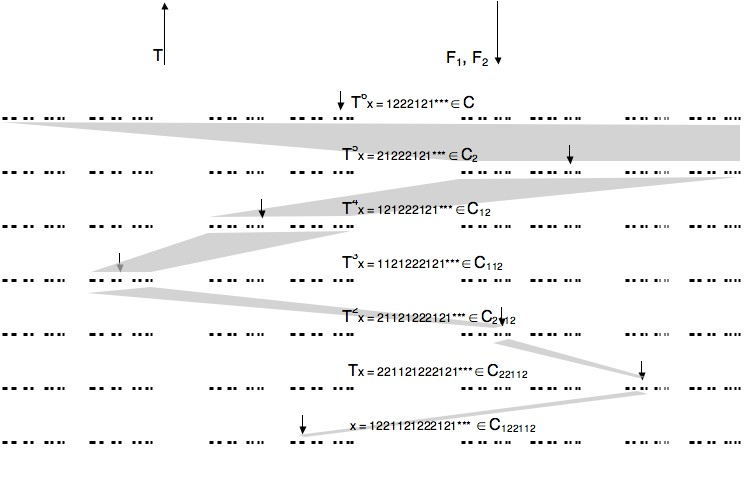
\includegraphics[width=14.7cm]{cantor2.jpg} 
   \caption{Nonlinear Cantor set, with IFS $ \{F_1,F_2\}$ and expansive map $ f=T $.}
   \label{cantor2}
\end{figure}

See Section  \ref{secpr} for pressure in a general dynamical system and Section~\ref{ssecpr} for pressure in the case of  subshifts of finite type.


%%%%%%%%%%%%%%%%%%%%%%%%
\subsection{The Underlying Set}
Suppose 
\[
E = E_1 \cup\dots \cup E_N \subset [0,1]
\]
is a Cantor set generated by a contractive IFS of nonlinear $ C^{1, \gamma } $ maps 
\[
 F_i:X \to X,\  X = [0,1],\ X_i = F_i (X) \text{ are mutually disjoint}
 \]
 For any word $ w $,
 \[
 X_w := F_w(X), \quad E_w := F_w (E) .
 \]
 
 \bigskip
 The expansive map $ f:X_1\cup\dots \cup X_N \to X $ has partial inverses $ F_i $, that is
 \[
 f(F_ix) := x.
 \]
For example, the $ F_i $ might be similitudes with contraction ration $ r_i $.  But we are interested here in the \emph{non}linear  case.

\bigskip
It is often convenient to identify $ E$ with the shift space $ \{ 1,\dots, N\}^{\mathbb{N} } $ by means of the usual addressing
\[  x = x_1x_2\dots \text{ if } x \in E_{x_1}\cap E_{x_1x_2} \cap\cdots .
\]
Then
\[ F_i(x) = ix_1x_2\dots, \quad f(x) = x_2x_3x_4\dots , \]
are right and left shift operators.

\bigskip Then $ (E,f) $ is a dynamical system and the \emph{orbit} of a point is  determined by its address, where the orbit of $ x $ is 
\[ 
x,\ f(x), \ f^2(x), \dots ,
\]
that is
\[ 
x_1x_2x_3\dots, \ x_2x_3x_4,\dots, \ x_3 x_4 x_5 \dots , \dots .
\]

\bigskip
As before, define
\[
S_k \phi  (x) := \sum_{i=0}^{k-1} \phi (f^i x),\quad e^{S_k \phi  (x) } 
   = e^{\sum_{i=0}^{k-1} \phi (f^i x)} = \prod _{i=0}^{k-1} e^{ \phi (f^i x)}.
   \]
Think of $  e^{S_k \phi  (x) }  $ as the product of weights along an initial segment of the orbit of $ x $.  

\bigskip 






%%%%%%%%%%%%%%%%%%%%%%%%
\subsection{Pressure Function}  This is a $ C^{0, \gamma } $ function $ \phi:E \to \mathbb{R} $, which is usually the restriction of some $ C^{0, \gamma } $ function  $ \phi :X_1\cup\dots \cup X_N \to \mathbb{R}  $.

The function $ \phi $ is usually used in the form of a multiplier or weight function $ g(x)= e^{\phi(x)} $, see Sections~\ref{secpr} and~\ref{ssecpr}.


\bigskip In this section, usually 
\begin{equation} \label{}
\begin{gathered}\label{ddfsk}
 e^{\phi(x)} = |Df(x)|^{-s}, \text{ i.e.\ }  e^{\phi(F_ix)} = |DF_i(x)|^s, \\
 e^{S_k\phi(x)} = |Df^k(x)|^{-s}, \text{ i.e.\ }  e^{S_k\phi(F_wx)} = |DF_w(x)|^s  \text{ if } |w|=k,
\end{gathered}
\end{equation} 
for some $ s $. Often $ s = \dim_{\mathcal{H}}(E) $ or $ s=1 $. 

 One goal of this approach is to   ``find''  the dimension of $ E $ for such nonlinear $ E $.
 
 \bigskip  The following proposition says:
  \begin{enumerate}
  \item The \emph{exponents} ($ S_k\phi(x) $ and $ S_k\phi(y) $) of weight growth of any two  orbits of the same length  $ k $   are equal up to an \emph{additive constant} ($ M$) independent of $ k $;
\item The \emph{weights}  ($ e^{S_k\phi(x)} $ and $ e^{S_k\phi(y)} $) of any two orbits  of  the same length length $ k $ are equal up to a \emph{factor} ($ e^M $) independent of $ k $;
  \item If the two orbits have the same coordinates  $ w=w_1\dots w_q $ for $ q > k $ then   the constant in the first case can be improved to  $M| f^k X_w| $ and in the second case to $ e^{M | f^k X_w|} $.
  \end{enumerate} 

\begin{proposition}[Bounded Variation] \label{PrBV}There exists a constant $ M $ such that if $ x,y\in X_w $ and $ |w|=k $ then  
\begin{equation} \label{rnrf} 
\big|S_k\phi(x) - S_k\phi(y) \big| \leq M, \quad \text{i.e.\  } e^{-M} \leq \frac{e^{S_k\phi(x)}}{e^{S_k\phi(y)}}\leq e^M .
\end{equation} 
If $ x,y\in X_w $ and $ |w|=q>k $ then 
\begin{equation} \label{}
\begin{gathered}
\big|S_k\phi(x) - S_k\phi(y) \big| \leq M |X_{w_{k+1}\dots w_q}| = M\left |f^k(X_w)\right|,\\
\text{i.e.\  } 
e^{-M\left |f^k(X_w)\right|} \leq \frac{e^{S_k\phi(x)}}{e^{S_k\phi(y)}}\leq e^{M \left |f^k(X_w)\right|}.
\end{gathered}
\end{equation}
\end{proposition} 

\begin{proof} Easy.  See Proposition~\ref{prpbv} or \cite{Fal}*{Prop 4.1, page 63}. \end{proof} 

%%%%%%%%%%%%%%%%%%%%%%%%
\subsection{Bounded Distortion} 

The following proposition says that if $ |w| = k $ then:
\begin{enumerate}

\item The map $ f^k:X_w \to X=[0,1]  $,  after rescaling its domain to have length one, has gradient (and hence Lipschitz bounds) bounded away from zero and infinity independently of the interval, and in particular \emph{independent of $ k $};
\item The inverse map $ F_w : X \to X_w $, after rescaling its range to have length one, has gradient (and hence Lipschitz bounds) bounded away from zero and infinity independently of the interval, and in particular \emph{independent of $ k $}.
\end{enumerate} 




\begin{proposition}  There exists a constant $ M $ such that for any $ k $, if $ |w|=k $, $ x,y \in X_w $ and $ z \in X $, then
\begin{gather*}
e^{-M} \leq |X_w|\, |Df^k(x)| \leq e^M, \\
\text{i.e.\ } e^{-M} \leq \frac{ |X_w|} {|DF_w(z)|} \leq e^M  , \\
e^{-M}|x-y| \leq |X_w|\,|f^k(x)-f^k(y)|\leq e^M|x-y|.
\end{gather*}
\end{proposition} 

\begin{proof} Since $ f^k:X_w \to X=[0,1] $, by the mean value theorem
\[
|Df^k(t)|=|X_w|^{-1} 
\]
for some $ t \in X_w $.
Hence taking $ e^\phi := |Df|^{-1}  $,
\[ e^{S_k\phi(t)} = |X_w|^{-1} \]
by  \eqref{ddfsk}.  From  \eqref{rnrf} with $ y=t $, the first two claims in the proposition now follow.

The last claim follows by the mean value theorem again.
\end{proof} 

\bigskip
\noindent Corollaries 4.3--4.6 in \cite{Fal} follow easily from the preceding proposition and state:
\begin{enumerate}

\item After rescaling $ X_w $ to have diameter one, the sets $ X_{w1} $ and $ X_{w2} $ are separated by a distance (bounded away from zero) independently of $ w $;

\item If $ x \in E_w $ and $ E $ is rescaled so $ |E_w|=1 $, then 
\[  E_w \subset B_1(x), \quad  B_\lambda (x) \cap (E\setminus E_w) = \emptyset, \]
for some $ \lambda $ independent of $ w $;

\item Suppose $ x \in E$ and $ r \leq r_0 $ (a  constant depending only on $ E $).  Then for some $ w $ with $ x \in X_w $ where $ |X_w| $ is comparable to $ r $ (up to factors depending only on $ E $), the map $ f^k:E\cap B_r(x) \to E $  is bi-Lipschitz  with Lipschitz bounds above and below comparable to $ r^{-1} $ (up to factors depending only on $ E $).

\item Suppose $ x \in E$ and $ r \leq r_0 $ (a  constant depending only on $ E $).  Then for some $ w $ with $ x \in X_w $ where $ |X_w| $ is comparable to $ r $ (up to factors depending only on $ E $), the map $ F_w:E\to E\cap B_r(x)   $  is bi-Lipschitz  with Lipschitz bounds above and below comparable to $ r $ (up to factors depending only on $ E $).

\item $   \dim_{\mathcal{H} }(E) = \underline{\dim}_B(E) = \overline{\dim}_B(E)=:s  $ and  $ 0 < \mathcal{H}^s(E) <\infty $. 

The equalities follow from either (3) and  \cite{Fal}*{Theorem 3.1}, or (4) and \cite{Fal}*{Theorem 3.2}.  The first inequality follows from  (3) and  \cite{Fal}*{Theorem 3.1}, the second from (4) and \cite{Fal}*{Theorem 3.2}.
\end{enumerate} 

%%%%%%%%%%%%%%%%%%%%%%%%%%%%%%%%%%%%










%%%%%%%%%%%%%%%%%%%%%%%%%%%%%%%%%%%%
%%%%%%%%%%%%%%%%%%%%%%%%%%%%%%%%%%%%
%%%%%%%%%%%%%%%%%%%%%%%%%%%%%%%%%%%%
\section{\textbf{Perron Frobenius Theorem}}   I mostly follow \cite{Boy} and~\cite{ Bri}*{pp 57--60}.  See also \cite{Boyd} for some comments and motivation.

%%%%%%%%%%%%%%%%%%%
\subsection{Basic Notions}
As in Section~\ref{secsp}, 
\begin{enumerate}

\item  A \emph{primitive} matrix is a square nonnegative matrix some power of which is positive.

\item An \emph{irreducible} matrix is a square nonnegative $ k\times k $ matrix $ A $ such that for every $1\leq  i,j \leq k $ there is a $ p $ such that $ {A^p}_{ij} $ is positive.
\end{enumerate} 

Note that ``primitive $ \Longrightarrow $ irreducible'' but not conversely.

We use the norm $ \|u\|= \sum_i |u_i| $, i.e.\  $ \|u\|= \sum_i u_i $ for nonnegative vectors $ u $, as is always the case here.

%%%%%%%%%%%%%%%%%%%
\subsection{Examples}\mbox{}
\begin{enumerate}
 
\item Let
\[
A=\begin{bmatrix}0&2\\1&1 \end{bmatrix}, \quad B=  \begin{bmatrix}0&4\\1&0 \end{bmatrix},
\]
then $ A^2 $ is positive and so $ A $ is primitive, while $ B $ is irreducible but not primitive.
  

\item \emph{Directed Graphs}.
Suppose $ A $ is a square nonnegative matrix and consider the graph with vertices $ \{1,\dots, k\} $  and a directed edge  $ ij $ iff $ A_{ij}>0 $.  

Then 
\begin{enumerate}

\item $ A $ is primitive iff for some $ p $ there is a path of length $ p $ between every ordered pair of vertices,
\item $ A $ is irreducible iff every ordered pair of vertices can be connected by a path (not all necessarily of the same length).
\end{enumerate} 

\item \emph{Stochastic Matrices}.  Suppose $ A=P $ is a stochastic (or Markov) matrix, i.e.\  $ P $, $ P_{ij}\geq 0 $ and $ \sum_j P_{ij} =1 $.   

The interpretation is that $ P_{ij} $ is the probability of going from node $ i $ to node $ j $ in one time step.  
 
 If $ x^{(0)} $ is the (probability) distribution at time $ 0 $ then $ x^{(0)}P $ is the distribution after one time step   and $ x^{(0)} P^n $ is the  distribution after $ n $  time steps.

\item \emph{Dynamic   Model}.  Here $ A $ determines an evolving mass.

For an  initial mass distribution $  x^{(0)} $ on $ \{1,\dots, k\} $, $ x^{(0)}A $ is the mass distribution after one time step   and 
\[
x^{(n)} :=  x^{(0)} A^n 
\]
 is the   mass distribution after $ n $  time steps.  

The total mass    is increasing at each time step  if $ \sum_j A_{ij} > 1 $ for all $i $, and is decreasing if  $ \sum_j A_{ij} < 1 $ for all $i $, and otherwise it depends on the mass vector $ [x_1,\dots, x_k] $. 

\item \emph{Population and Economic Models}. The mass $ x^{(n)}_i$ in (4) could be interpreted in a \emph{population model} as the number of individuals in group $ i $, and in an \emph{economic model} as the activity level, or resources produced, in sector $ i $.
\end{enumerate} 
 

%%%%%%%%%%%%%%%%%%%%%%%%%
\subsection{Interpretation}  One can probably best  interpret the following theorems in terms of the previous dynamic model.

\medskip If $   x $ is a mass distribution on $ \{1,\dots, k \} $, i.e.\  $ x =[x_1,\dots, x_k] \in \mathbb{R}^k $ with $ x_i \geq 0 $, then $ \|x\| $ is the \emph{total mass} of $x $. 

If $ x $ is the mass distribution   at one time step,  then $ x A =   [(x A)_1,\dots (x A)_k] $ is the mass distribution at the next time step.

Since $ (x A)_j = \sum_ix_i A_{ij} $,  $ A_{ij} $ is interpreted as the proportion or multiple of mass at  $ i $ which is moved to $ j $ at the next time step.  Unlike in the stochastic case we allow $ \sum_j A_{ij} \neq 1 $, i.e.\ we do not assume conservation of mass.  As noted before, the mass   at  node $ i $  is increasing at each time step  if $ \sum_j A_{ij} > 1 $, and is decreasing if  $ \sum_j A_{ij} < 1 $.  

\medskip
In order to interpret  multiplication of $ A $ by a vector on the \emph{right},   consider a \emph{weight function} (value function, utility function, price system)
\[
y = \begin{bmatrix} y_1 \\ \vdots \\ y_k \end{bmatrix} = [y_1,\dots, y_k]^t , 
\]
with values depending on the ``position'' $ i \in \{1,\dots, k\} $.   Then the corresponding \emph{total  weight} (total value, total utility, total price) of the mass distribution $ x $ is $ \langle x,y \rangle = \sum_ix_i y_i $. 

The weight function $ y $ can be quite arbitrary, although normally nonnegative.  For example, consider a markov chain $ P=A $ determining the flow of taxis between three locations in a city.  The weight function for a resident  
living near the first node could possibly look like $ [1, 1/3, 1/4] $.  Multiplying through by a scalar is essentially just a change of units.

\medskip Since 
\[
\langle x, Ay \rangle = \langle x A, y \rangle,\ ( \text{i.e.\ } \langle A^t x, y \rangle ),
\]
one interprets  $ Ay $ as the weight function which acts on an arbitrary mass distribution $ x $ in such a way that the total weight of $ x $ under $ Ay $ is the same as the total weight of  the evolved mass distribution $ xA  $ under $ y $.

Since  $ (Ay)_i = \sum_jA_{ij}y_j $,   $ A_{ij} $ can also be interpreted as  the multiplier of the weight (or price) function at $ j $ which is added to the price at $ i $ to obtain $ (Ay)_i  $.

\medskip
In terms of a directed graph with weights $ A_{ij} $ on the edge \emph{from} $ i $ \emph{to} $ j $, note  that the mass component $ (x A)_j$ is obtained from the multipliers   on the arrows pointing \emph{into} $ j $, whereas the weight (or price) component $ (Ay)_i $ is obtained from the multipliers on the arrows pointing \emph{out of}~$ i $.

\medskip  To interpret the following Perron Frobenius theorem, first note that it applies equally to $ A $ and $ A^t $.

Suppose 
\[
 uA = \lambda u, \quad  Av= \lambda v  .
 \]

Note that for a stochastic matrix, $ \lambda = 1 $, $ u $ is the unique steady state probability (mass) distribution, and $ v = [1,\dots, 1]^t $.  

More generally, $u $ is the unique (up to  scalar multiples) steady state mass distribution modulo rescaling.  The rescaling factor $ \lambda$ is the   total mass multiplier, i.e.\  $ \|uA\| = \lambda \|u\|$.
Similarly, $ v $ is the unique (up to scalar multiples) steady state weight function (price functions) modulo rescaling, and the rescaling is by the same multiplier $ \lambda $.

If $ \beta $  is any other eigenvalue of $ A$ or $ A^t $ then $ | \beta | < \lambda $.   Any right e-vector $ y $ can be written uniquely as  
\[
y =\alpha v + z , \text{ where } z \in \ker u, \text{ i.e.\ } \langle u,z \rangle = 0,
\]
in fact $ \alpha = \langle u,y \rangle / \langle u,v \rangle $.  Moreover, $ \ker u $ is invariant under $ A $, and so the e-values on $ \ker u$ have modulus $ < \lambda $.

It follows that asymptotically
\[ 
A^n \sim \lambda ^n \langle u,v \rangle ^{-1}v \otimes u ,
\]
since $  \langle u,v \rangle ^{-1}v \otimes u $ is just projection onto $ v $ with kernel $ \ker u $.

%%%%%%%%%%%%%%%%%%%%%%%%
\subsection{Main Theorem}
 

 A result analogous to the following is also true in the irreducible case.  See \cite{Boy} and~\cite{ Bri}*{pp 57--60}.  But the main ideas in the proof are already contained in the primitive matrix case.

\begin{theorem}[Perron Frobenius] \label{pft} Suppose $ A $ is primitive.  Then there exists a positive eigenvalue $ \lambda $ such that
\begin{enumerate}
\item $ \lambda  $ is a simple root of the characteristic polynomial %
\footnote{The characteristic polynomial is $ \det (A-xI) $.  The roots $ \lambda $ are the eigenvalues of $ A $.  The algebraic multiplicity of $ \lambda $ equals  the geometric dimension  of the   \emph{generalised} eigenspace corresponding to $ \lambda $, and  so is $ \geq $ the geometric dimension of the eigenspace corresponding to  $\lambda $.}
(so in particular the corresponding eigenspaces for $ A $ and $ A^t $ are one dimensional),
\item $ \lambda  > |\tau| $ if $\tau $ is any other root %
\footnote{\label{arot}Since the coefficients of the characteristic polynomial are real the complex roots come in conjugate pairs.  Suppose $ re^{i\theta} $ is a complex eigenvalue with eigenvector $ w \in \mathbb{C} ^k $.  Let $ w_1 $ and $ w_2 $ be the  real and imaginary parts of $ w $.  Then  taking real and imaginary parts of $ Aw =  re^{i\theta} w $ we  see  in the real 2-dimensional space spanned by $w_1 $ and $ w_2$ that $ A $ is a rotation by $ \theta $ followed by a stretch with $ r $.} 
(so  in particular the spectral radius  of  $ A $ is $ \lambda $),
\item $ A $ has a positive eigenvector $ v $ for $ \lambda $ (and similarly for its transpose $ A^t $), 
\item $ A $ has no nonnegative eigenvectors other than multiples of $v  $  (and similarly for $ A^t $).  
\item   $ \min_i \sum_jA_{ij} \leq \lambda \leq \max_i \sum_j A_{ij} $.
\item Suppose    $ x \geq 0 $.   Then $ Ax < \gamma x \Longrightarrow \lambda < \gamma  $ and $ Ax > \gamma x \Longrightarrow \lambda > \gamma  $.
\end{enumerate} 
\end{theorem} 

\begin{proof}\mbox{}

\noindent \textbf{1}.  \emph{Lemma}: \emph{Suppose $ L: \mathbb{R}^k \to \mathbb{R}^k $ is linear, $ K $ is compact, $ 0 \in K^\circ $ (the interior of $ K $), and $ L^i(K)\subset K^\circ$ for some $ i >0 $.  Then $ \lambda $ is an eigenvalue of $ L $ implies $ | \lambda | < 1 $.}

To see this consider two cases.

If $   | \lambda | > 1 $ then iterates of $ L $ send eigenvectors to $ \infty $, contradicting $   0 \in S^\circ $ and the fact $ L^j(K^\circ) $ is bounded independently of $ j $.

If $ |\lambda| = 1$ consider a corresponding 2-dim subspace $ V $ on which $ L $  acts as a rotation, see footnote~\ref{arot}.  Consider some $ v \in \partial K \cap V $. Either some iterate of $ L $ sends $ v $ to itself, or iterates of $ L $ applied to $ v$ are dense in the unit circle for the subspace $ V $.  Both  contradict  $ L^i(K)\subset K^\circ$.

\medskip \noindent \textbf{2}. Let $\|v\|= \sum_i|v_i| $ for $ v = (v_1,\dots, v_n) \in \mathbb{R}^n$.
  Since $ A $ is nonnegative the map $ f(x) = Ax/\|Ax\| $ sends the unit simplex into itself.  By the Brower fixed point theorem there is a fixed point $ v $, and $ v $ is  then a  nonnegative eigenvector of $ A $ with   eigenvalue $ \lambda >0$.  Since some iterate of $ A $ is positive, $v  $ is positive.

This proves (3).


\medskip \noindent \textbf{3}.  Use $ v $ and $ \lambda $ to transform $ A $ to a  \emph{stochastic}  (i.e.\ probability)  matrix $ P $ with right eigenvector $(1,\dots, 1)^T $ and eigenvalue $ 1 $.   That is
\begin{equation} \label{dfPA}
P := \lambda ^{-1} V^{-1} A V, \text{ or equivalently } P_{ij} = \frac{A_{ij}v_j}{\lambda v_i} = \lambda ^{-1}\frac{v_j}{v_i} A_{ij},
\end{equation} 
where $ V $ is the diagonal matrix with entries from $ v $.   That is, rescale the axes to obtain a coordinate change so that   $ v $ becomes  the unit vector, and then rescale $ A $ so the corresponding  eigenvalue is  one.

Note that 
\begin{align*} 
0\leq P_{ij}, \quad \sum_j P_{ij} = 1,\\
\lambda ^{-n}  \det(A-\tau I) &= \det( P-\lambda ^{-1}\tau I) \\
Av = \tau v \Longleftrightarrow  P(V^{-1}v) &= \lambda ^{-1}\tau\, V^{-1}v 
\end{align*} 

\medskip \noindent \textbf{4}. It is now sufficient to prove (1) and (2) for $ P $, with $ \lambda   $ replaced by $ 1 $ and corresponding  e-vector $ (1,\dots,1)^T  $.  In fact we will prove  (1) and (2)  for   the transpose $ P^t $, i.e.\ for the left action of $ P $. 

First note that the \emph{transpose} $ P^t $ maps the unit simplex $S $  into itself.  Let $ w \in S $ be the unique nonnegative left e-vector with eigenvalue one for $ P^t $.%
\footnote{This eigenvector exists either from \textbf{1} applied to the transpose of $ P $, or by the standard markov chain result for the existence of a stationary probability distribution.}


 Consider the translate $ S - w $. Then $ P^t :S-w\to S-w $.
 
 Working in the codimension one subspace spanned by $ S-w $ we can apply step \textbf{1}   to $ P^t $, noting that since for some power of $ P^t $ all entries are positive,  this power maps $ S-w $ to its interior.  Hence all eigenvalues of $  P^t $ restricted to this subspace are strictly less than 1.  The remaining e-value and e-vector of $ P^t $ are $ 1 $ and $ w $. 
 
 This gives (1) and (2) for $ P^t  $, and hence for $ P $, and hence   for $ A $.
 
 \medskip \noindent \textbf{5}.   To prove  (4) suppose $ w  $ is a nonnegative e-vector of $ A $ with e-value $  \beta$.  Since $ A^i w = \beta ^i w $ and the left side is positive for some $ i $, it follows $ w $ is in fact positive and so $ \beta $ is real and positive.  Also, $ \beta \leq \lambda $ since $ \lambda $ is the spectral radius.
 
 Suppose $ v $ is a positive e-vector corresponding to the   e-value $ \lambda $ and choose a positive e-vector $ w $ for $ \beta $ such that $ w>v $ componentwise.   
 Then $ A^iw >  A^iv $ for all $ i $, hence $ \beta ^i w > \lambda ^i v $ for all $ i $, which is impossible if $ \beta < \lambda $.
 
Hence $ \beta = \lambda $.  Since  $ \lambda $ is a simple root of the characteristic equation the corresponding eigenspace is one dimensional and so we are done.

 \medskip \noindent \textbf{6}.  For (5) let $ v_p = \min\{v_1,\dots v_k\}$. Then
 \[
 \lambda v_p = \sum_j A_{pj} v_j \geq \bigg( \sum_j A_{pj} \bigg) v_p \geq \bigg( \min_i \sum_p A_{ij}\bigg) v_p.
 \]
 Similarly for $ \max $.
 
 \medskip \noindent \textbf{7}.    Suppose $ Ax < \gamma x $ for some $ x \geq 0 $. It follows $ \gamma > 0 $ and so $ x > 0 $.
 
 W.l.o.g.\ suppose $ v<x $ where $ Av = \lambda v $.  Note $ v>0$.
 
 Then for all $ n $, 
 \[
 \lambda ^n v = A^n v < A^n x < \gamma ^n x.
 \]
 This is impossible if $ \gamma < \lambda $, hence $ \lambda \leq \gamma $.
 
 But $ Ax < \gamma x $ and $ x>0 $ implies $ Ax < (\gamma- \epsilon) x $ for some $ \epsilon > 0 $.
 Hence $ \lambda \leq \gamma - \epsilon  $ and so $ \lambda < \gamma $.   
 
  A similar proof applies if $ Ax > \gamma x $ for some $ x \geq 0 $.
 \end{proof} 


\begin{remark}
***to be checked***  The fact that $ P $, defined by ``normalising'' $ A $  by its right eigenvector as in \eqref{dfPA}, is a stochastic matrix, is 
important in understanding the Ruelle Perron Frobenius theorem, particularly the existence of a \emph{shift invariant} equilibrium measure.  

*** (Need normalising here) *** It is easily checked that the left e-vector $ \pi $ of $  P $ is the same as the left e-vector $ u $ of $ A $ \emph{weighted} by its right e-vector $ v $, which is the same as the diagonal vector of $v\otimes u/\langle u,v \rangle  $, see~\eqref{limA}.   That is,
\[
\pi = (u_1v_1,\dots, u_kv_k) .
\]
Of course, the right e-vector if $ P $ is just $ (1,\dots, 1) $.
\hfill $\square$  \end{remark} 


%%%%%%%%%%%%%%%%%%%%%%%%%%%%
\subsection{Limit Theorem}
\begin{corollary}\label{corlt}
  Suppose $ A $ is primitive, $  \lambda  $ is the spectral radius, $ u  $ is a
 left (row) e-vector for $ \lambda   $, and $ v $ is a right (column) e-vector for $ \lambda   $.

Then 
\begin{equation} \label{limA} 
  \lambda ^{-n}A^n \to \frac{v\, u }{u  v}  = \frac{v \otimes u}{  \langle u , v \rangle } ,
\text{ i.e.\ }  \lambda ^{-n}A^n w \to   \frac{ \langle u , w \rangle}{  \langle u , v \rangle }\, v ,
   \text{ exponentially fast as } n\to \infty ,
\end{equation} 
  where $ v  u  = v\otimes u $ is the rank one $ k \times k $ matrix obtained by multiplying the column vector  $v  $ by the row vector~$ u$, and $ uv = \langle u , v \rangle $ is the scalar obtained from matrix multiplication in the reverse direction.
\end{corollary}


\begin{remark}\mbox{}

\begin{enumerate}
\item The matrix $ \dfrac{v\, u}{uv} $ is projection onto the subspace spanned by $ v $ whose kernel is the codimension one subspace annihilated by $ u $.

\item W.l.o.g.\  we \emph{normalise} the e-vectors $ u $ and $ v $ so 
\[
\|u\|:= \sum_i|u_i| = 1 , \quad  u v = \sum_i u_i v_i =1 , 
 \]
 \item 
In particular,  $  \lambda ^{-n}A ^n   \to  v \, u $ and  $  \lambda ^{-n}A ^n_{ij}  \to  v_i\, u_j $, exponentially fast. 


\item  Taking norms, $   \lambda  ^{-n} \|A\|^n \to \|v\, u\| $.  Taking logs and dividing by $ n $, 
\[   \lim_{n\to \infty} \frac{1}{n} \log \|A^n\| =  \lambda . \]

\item It follows from (3) that
\begin{align*}
\lambda ^{-n} x^{(n)} &\to \langle x^{(0)},v\rangle\, u ,  \quad \text{since } x^{(n)} = x^{(0)} A^n, \\
\lambda ^{-n} \|x^{(n)}\| &\to \langle x^{(0)},v\rangle,  \quad \text{since }  \|u\|=1,  \\
\frac{x^{(n)}}{\|x^{(n)}\|}  &\to u, \quad \text{from the preceding two limits},     \\
\frac{x^{(n+1)}_i}{ x^{(n)}_i}  &\to \lambda,  \quad \text{from the first limit} . 
\end{align*} 

\item The first limit above says the asymptotic distribution is  $ u $ scaled by $ \langle x^{(0)},v\rangle  $.
The second says the asymptotic total mass is $ \langle x^{(0)},v\rangle $.

If $ v $ is the vector of units as in the stochastic case then $ \langle x^{(0)},v\rangle = \sum_i x^{(0)}_ i  $.
In general the \emph{interpretation of $ v $} is that it gives the contribution of each component of $  x^{(0)}$ to the asymptotic mass distribution.   

The \emph{interpretation of $ u $} by the third limit is as  the limit of the normalised distributions.  For the Markov case it is the steady state probability distribution.

The fourth limit says that the one time step limit growth factor in every component is $ \lambda $.
\end{enumerate} 
\end{remark}

\begin{proof}[Proof of Corollary] W.l.o.g.\ take $ \lambda=1 $ by multiplying $ A $ by a constant.  Then all other e-values have modulus less than $ 1 $.

Choose a basis such that  $ A $ is in Jordan normal form with  $ 1 $ the top left entry and all other diagonal entries strictly less than $ 1 $ in modulus.  

Since $ 1 $ is a simple root of the characteristic equation, all entries in  the left column and top row other than the unit diagonal element must equal zero.  It follows by uniqueness of the left and right eigenspaces corresponding to $1  $ that in the new basis $ u= (1,0,\dots, 0) $ and $ v= (1,0,\dots, 0)^t $.

Moreover, since all diagonal elements are less than one in modulus,  it is easy to check that powers of any submatrix corresponding to any other generalised e-space converges exponentially fast to $ 0 $.  For example, 
\[
B = \begin{bmatrix} \beta &1 &0 \\ 0 &\beta & 1 \\ 0 & 0 & \beta \end{bmatrix}, \quad
B^2 = \begin{bmatrix} \beta^2 &2 \beta  &1 \\ 0 &\beta^2  & 2 \beta  \\ 0 & 0 & \beta^2 \end{bmatrix}, \quad
B^3 = \begin{bmatrix} \beta^3 &3 \beta^2  &3 \beta  \\ 0 &\beta^3  & 3 \beta^2  \\ 0 & 0 & \beta^3 \end{bmatrix}, 
\quad \text{etc.}
\]

Hence $ A^n $ converges exponentially fast to the matrix with $ 0 $ everywhere except for $ 1 $ in the top left corner.  Thus for  this coordinate system, $ A^n \to v\,   u^t $.   Since the assertion is independent of the coordinate system,  we are done.
\end{proof} 


%%%%%%%%%%%%%%%%%%%%%%%%%%%%%%%%%%%%
%%%%%%%%%%%%%%%%%%%%%%%%%%%%%%%%%%%%
%%%%%%%%%%%%%%%%%%%%%%%%%%%%%%%%%%%%
\section{\textbf{Graph Directed IFS}}   

We apply the Perron Frobenius theorem to find the dimension of a graph directed IFS with similitudes and satisfying the open set condition.  See \cite{Fal}*{pp 48--51, Ex 3.7 p57} and \cite{Edg}*{pp 190--1,  pp 172--3}.%
\footnote{Falconer first does the box dimension, then assumes a strong separation condition to get the Hausdorff dimension case from the scaling type  \cite{Fal}*{pp 42--45, Theorems 3.1 and 3.2}.  

Edgar has a proof spread throughout the book, using ``Method I'' in Chapter 5 to construct the relevant measure, pp 190--1 for properties of the associated matrix, and pp 172--3 for applying the open set condition.

Mauldin and Williams \cite{MW} use a fair amount of the thermodynamic formalism.}


\begin{figure}[htbp] %  figure placement: here, top, bottom, or page
   \centering
   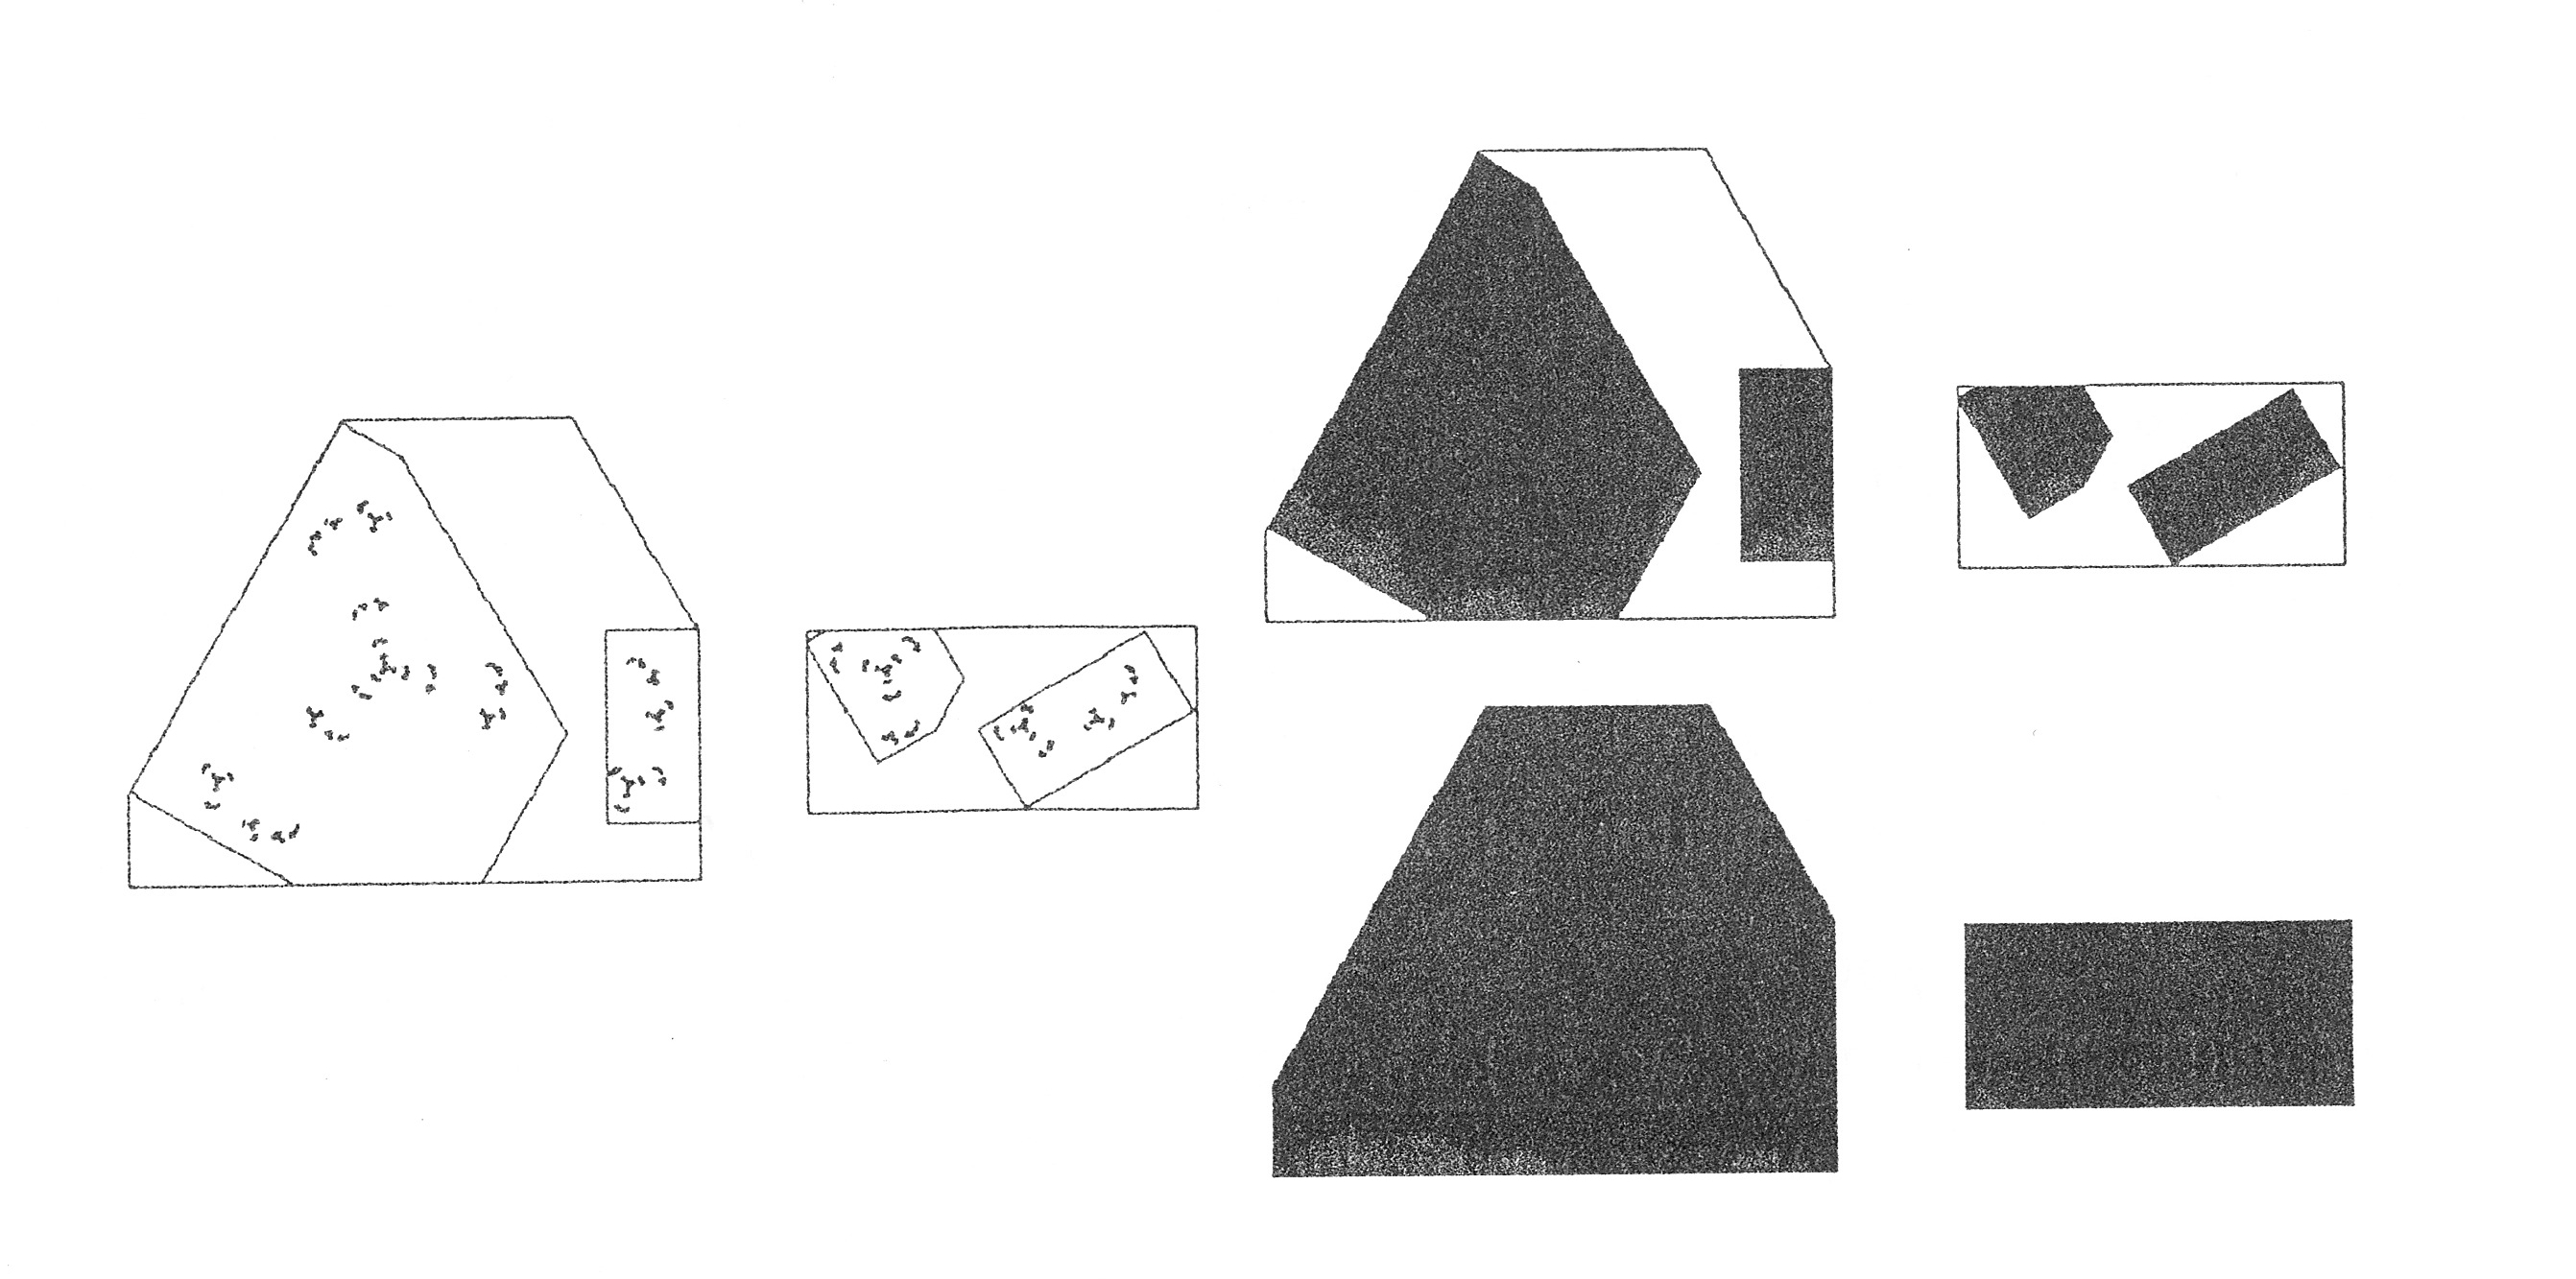
\includegraphics[angle=180, width=6in]{osc.jpg} 
   \caption{Open set condition for a graph directed IFS.  From~\cite{Edg}*{p 169}.}
   \label{osc}
\end{figure}

%%%%%%%%%%%%%%%%%%
\subsection{Directed Graph}  

\begin{definition} A \emph{directed graph} is a pair $ (V,E) $ where $ V =\{1,\dots, k\}$ is the set of vertices and $ E $ is the set of directed edges.  
\begin{align*}
E_{ij} &= \text{set of edges from $ i $ to $ j $},\\
E_{ij}^p &= \text{set of paths of length $ p $ from $ i $ to $ j $}.
\end{align*} 
We assume the \emph{transivity condition}: for any pair $ (i,j)$ of vertices there is a path from $ i $ to $ j $.
\end{definition} 
There may be more than one edge from $ i $ to $ j $.

Each edge $ e $  will later correspond to a function $ f_e $.  The composition $ f_e\circ f_{e'} $ is admissable iff the ``head'' vertex for $ e $ is the same as the ``tail'' vertex for $ e' $.

\begin{remark}  Contrast this with the set-up in Section~\ref{PFT}, where each \emph{vertex} $ i$ corresponds to a function $ f_i $.  The composition $ f_i\circ f_j $ is admissable iff there is an edge from $ i $ to $ j $.  There is at most one edge from $ i $ to $ j $. 

For a standard IFS with $ k $ maps the current model leads to a graph with $ 1 $ vertex and $ k $ edges from this vertex back to itself.  The previous model leads to  a graph with $ k $ vertices and a directed edge from every edge to every edge, including itself, i.e.\ $ k^2 $ edges.
\end{remark}

 
%%%%%%%%%%%%%%%%%%
\subsection{Graph Directed IFS}  See Figure~\ref{osc}.

\begin{definition} \label{gdifs}   A \emph{graph directed IFS} associated  with the directed graph $ (V,E) $ is a set of contractive similitudes $ F_e:\mathbb{R}^m \to \mathbb{R}^m $ where  $ e\in E $ which satisfies the open set condition.  That is, there are nonempty open sets $ U_i $ for $ i \in V $ such that 
\begin{align*}  
e \in E_{ij}  &\Longrightarrow F_e(U_j)\subset U_i, \\
e\in E_{ij}, \ e'\in E_{ij'},\  e \neq e' &\Longrightarrow F_e(U_i) \cap F_e(U_j) = \emptyset.
\end{align*} 
The Lipschitz constant for $ f_e $ is denoted by $ r_e $.
\end{definition}

\begin{proposition}\label{gdd}
 For a graph directed IFS as in Definition~\ref{gdifs} there exists a unique family $\{ K_1,\dots K_k\} $ of compact sets such that 
\[
K_i = \bigcup_{j=1}^k \bigcup_{e\in E_{ij}} F_e(K_j) .
\]
Moreover, for any $ n $,
\[
 K_i = \bigcup_{j=1}^k \bigcup_{(e_1,\dots, e_n) \in E^n_{ij}} F_{e_1}\circ \dots \circ F_{e_n}(K_j) .
 \]
 
 \end{proposition}
 
\begin{proof}  Standard using the contraction mapping principle and the Hausdorff metric. \end{proof} 
 
 %%%%%%%%%%%%%%%%%%
\subsection{Associated Matrices}  For $ s > 0 $ define the matrix $ A(s)$ by
\[   A(s)_{ij} := \sum_{e\in E_{ij}} r_e^s . \] 
Then $ A(s) $ is nonnegative, and irreducible by the transitivity of $ (V,E) $.

Let  $ \lambda (s) $ 
be the largest (real) eigenvalue of $ A(s)$, given by the Perron Frobenius theorem. (We only proved the primitive case).

\begin{proposition} \label{ev1} Under the above assumptions on $ (V,E) $, the e-value $  \lambda(s) $ is continuous  and strictly monotone decreasing.  Moreover,
\[
\lambda(0)\geq 1,  \quad \lambda(s)\to 0 \text{ as } s \to \infty .
\]
In particular, there is a unique $ d\geq 0 $ such that $ \lambda(d) = 1 $.
\end{proposition} 

\begin{proof}  We use Theorem~\ref{pft}(6).

\medskip Since there is at least one entry in each row of $ A(0) $, for any $ \epsilon > 0 $,  
\[ A(0)\boldsymbol{1} \geq \boldsymbol{1} > (1-\epsilon)  \boldsymbol{1} .
\]
Hence $ \lambda (0)> (1-\epsilon ) $ and so $ \lambda(0) \geq 1 $.

\medskip
Since $ A(s) \boldsymbol{1} \leq \epsilon \boldsymbol{1} $ for all $ s $ sufficiently large, $ \lambda (s) \leq \epsilon $ and so $ \lambda(s)\to 0 \text{ as } s \to \infty $.

\medskip Let $ A(s)\, v(s) = \lambda (s)\, v(s) $. Then
\begin{align*}
A(t )\, v(s) &= A(s)\, v(s) + \big( A(t ) - A(s) \big) v(s) \\
   &= \lambda (s) v(s) + o(|s-t| ) v(s) \\
   &\leq ( \lambda(s) + \epsilon ) v(s) 
\end{align*}
for all $ t $ such that $ |s-t| $ is sufficiently small.  Hence 
\[
\lambda(t)\leq \lambda(s) + \epsilon 
\]
and similarly 
\[
\lambda(t)\geq \lambda(s) + \epsilon 
\]
for all $ |s-t| $ sufficiently small. This give s continuity.

\medskip Note 
\[
\frac{d}{ds}A(s)_{ij} \leq 0, \quad \frac{d}{ds}A(s)_{ij} < 0 \text{ unless } A(s)_{ij} \equiv 0 .
\]
Hence for $ A(t)\, v(t) = \lambda (t)\, v(t)$,
\[
s > t \Longrightarrow A(s)\, v(t) < A(t)\, v(t) = \lambda (t)\, v(t).
\] 
Hence $ \lambda(s) < \lambda (t ) $. 
\end{proof} 
 
 %%%%%%%%%%%%%%%%%%
\subsection{The Dimension Theorem}  

\begin{remark}
 \emph{Motivation}: By transitivity, if $ i \neq j $ then  $ K_i $ contains a scaled copy of $ K_j $ at some level.  It follows the $ K_i $ all have the same dimension, and if $ 0<\dim K_i <\infty $ for some $ i $ then the same is true for every $ i $.

If in addition the unions in Proposition~\ref{gdd} are disjoint and $ s $ is the dimension of each $ K_i $, then
\[
\mathcal{H} ^s(K_i) = \sum_{j=1}^k \sum_{e \in E_{ij}} r_e^s \mathcal{H} ^s(K_j) 
   = \sum_{j=1}^k A(s)_{ij} \mathcal{H} ^s(K_j) ,
   \]
Hence $\big(\mathcal{H} ^s(K_1), \dots,  \mathcal{H} ^s(K_k)\big) $        is the unique positive right e-vector 
of $ A(s) $ and its e-value is one.
  \end{remark}

\begin{theorem} Suppose $\{ K_1,\dots K_k\} $ is the attractor of the graph directed IFS in Definition~\ref{gdifs}. (Note that the $ F_e $ are similitudes and the open set condition is assumed).  Suppose $ d $ is as in Proposition~\ref{ev1}. 


Then $ 0 <  \mathcal{H} ^d (K_i ) <\infty $ for all $ i $, and in particular $ \dim_{\mathcal{H}}(K_i ) = d $. 
\end{theorem}

\begin{proof}
Let $ v $ be the unique right e-vector for $ A:=A(d ) $ and note that the e-value is  one.  

Build a measure on   each $ K_i $ by successively assigning a mass to the admissable $  F_{e_1}\circ \dots \circ F_{e_n}(K_j)$ as follows.

\begin{enumerate}

\item Assign   mass $ v_i $ to each $ K_i $.

\item Assign   mass $ r_e^d  v_j $ to $ F_e(K_j) $ if $ e \in E_{ij} $ for some $ i $, and hence mass
$  A_{ij} v_j$ to $K_{ij} := \bigcup_{e\in E_{ij}} F_e(K_j) $.  (Note $  K_{ij} = \emptyset $ iff  $ A_{ij} = 0 $.)

This is compatible with the previous assignment since $ v $ is a right e-vector of $ A $ with e-value one.

\item Assign mass $ r_{e_1}^d  \cdots  r_{e_n}^d v_j $ to $ F_{e_1}\circ \dots \circ F_{e_n} (K_j) $ if $ j $ is the terminial vertex for $ e_n $, and hence mass
\[
A_{i_0i_1}\cdots A_{i_{n-1}i_n} v_{i_n} \text{ to } K_{i_0i_1\dots i_n} :=
  \bigcup F_{e_1}\circ \dots \circ F_{e_n} (K_{i_n}),
  \]
 where the union is over all $ (e_1,\dots, e_n) $ such that $ e_1 \in E_{i_0i_1}, \dots, e_n \in E_{i_{n-1}i_n} $. 

Again, this is compatible with previous assignments since $ v $ is a right e-vector of $ A $ with e-value one.
\end{enumerate} 

In this manner one obtains a measure $ \mu $ on $K := \bigcup_i K_i $.  

Moreover, given  $ r> 0 $ we truncate each allowable infinite sequence of edges to $ e_1 \dots e_n $  in the usual manner so that   the product of the  corresponding $ r_{e_i} $  is comparable to $ r $. The value   of $ n $ depends on the sequence and on $ r $. 

Suppose $ x \in K$. A uniformly bounded number of such $ F_{e_1}\circ \dots \circ F_{e_n} (K_j) $ meet $  B_r(x) $ by a volume comparison argument.  

This gives $ \mu (B_r(x) ) \leq cr^d $ and hence by the mass distribution principle $ \mathcal{H} ^d  (K_i) > 0 $ for each~$ i $.

An upper bound $   \mathcal{H} ^d  (K_i) < \infty  $ follows from the definition of $  \mathcal{H} ^d $ and using covers $ F_{e_1}\circ \dots \circ F_{e_n} (K_j) $.
\end{proof}  


%%%%%%%%%%%%%%%%%%%%%%%%%%%%%%%%%%%%
\section{\textbf{Ruelle Perron Frobenius, Special case}}  This is motivated by~\cite{Kea}.

Let $ (X,T) $ be a subshift (of finite type) of the full shift on $ \Sigma_k $ which is given by the adjacency matrix $ \widetilde{A} $.  

Let  $ \phi $ be a pressure function such that $ \phi(x) $ depends only on the first two coordinates $ x_0x_1 $. Equivalently, $ \phi $ is given by a matrix
\begin{equation} \label{dfA} 
A_{ij} = \begin{cases} e^{\phi(ij)} & \widetilde{A}_{ij} \neq 0 \\
                                              0  &  \widetilde{A}_{ij}= 0.
              \end{cases}.
\end{equation} 
 
 Note that $ A $ is primitive iff $ \widetilde{A} $  is primitive.  Moreover, any nonnegative matrix $ A $ with this property is of the given  form. 
 
 Clearly, $  \phi $ is H\"{o}lder continuous.
 
\medskip Let $ \lambda $  be the positive e-value for $ A $ with positive left and right e-vectors $ u $ and $ v $. Let $ P $ be the associated stochastic matrix with left e-vector $ \pi $.  That is, 
\begin{equation} \label{dfda} 
u^TA = \lambda u^T, \quad Av = \lambda v , \quad \|u \|=1, \quad \langle u,v \rangle = 1,
\quad P_{ij} = \lambda ^{-1}\frac{v_j}{v_i} A_{ij}, \quad \pi_i  = u_i v_i.
\end{equation} 
We will find the pressure and certain Gibbs measures for $ \phi $ in terms of these quantities.

%%%%%%%%%%%%
\subsection{Pressure}  From~\eqref{defw},
 \[
 e^{ S_n \phi  (a) }\sim w([a_0\dots a_{n-1}]) \sim A_{a_0a_1}\cdots A_{a_{n-1}a_n},
 \]
 where ``$ \sim $'' means well-defined and/or equal up to a factor $ M $ independent of $ n $. 
 Choosing any $ j $ and setting $ a_n = j $,  by Corollary~\ref{corlt}
 \[
 \sum_{a_0,\dots, a_{n-1}} w([a_0\dots a_{n-1}]) = \sum_{i,j=1}^k A^n_{ij} \sim \lambda ^n.
 \]
It follows from Definition~\ref{dfpg} that 
\[
 P(\phi) = \lambda .
 \]

%%%%%%%%%%%%%%%%%%%%%%%%%% 
 \subsection{IFS invariant Gibbs measure}  From the definition~\eqref{defw} of a weight function it is natural to look here for a Gibbs measure $ \mu $ which reflects the structure of this definition, and in particular is such that
\begin{equation} \label{pfi} 
\begin{aligned} 
   \mu([a_0a_1\dots a_{n-1} ]) &= \lambda ^{-1} A_{a_0a_1}\mu([a_1\dots a_{n-1}  ]) ,\\
  \text{i.e.\ } \mu([a_1\dots a_{n-1}  ]) &= \lambda \big(A_{a_0a_1}\big)^{-1} \mu([a_0a_1\dots a_{n-1} ]) .
\end{aligned}
\end{equation} 
  
  Accordingly, define $ \mu $ on cylinder sets by
 \begin{equation} \label{dfmu} 
 \mu([a_0]) = v_{a_0}, \quad 
  \mu([a_0\dots a_{n-1}])= \lambda ^{-(n-1)} A_{a_0a_1}\cdots A_{a_{n-2}a_{n-1}} v_{a_{n-1}}
  \text{ if } n\geq 2.
 \end{equation} 

Then  $ \mu $ satisfies the compatibility condition
  \[
   \mu([a_0\dots a_{n-1}]) = \sum_j   \mu([a_0\dots a_{n-1}j]) 
   \]
   because $ v $ is a right e-vector for $ \lambda $.  Hence $ \mu $ defines a measure on  $ X $.  It is clearly a Gibbs measure from \eqref{dfgm}, \eqref{defw}, \eqref{dfA} and the fact $ P(\phi) = \lambda $.  

By multiplying  $ \mu $ by a $ \|v\|^{-1} $  we could take  $ \mu$  to also be a probability measure.  But this is probably not so natural in light of Remark~\ref{norch}. 

\medskip To see carefully that \eqref{pfi} implies $ \mu $ is IFS invariant in the sense $ L^*_g(\mu) = \lambda \mu $, see Section~\ref{secam}, we use Proposition~\ref{lgpf}.  So we w.t.s.\ $ \sum_iF_{i\#}(\text{w}_i\mu) = \lambda \mu $.

Compute 
\begin{align*}
\sum_iF_{i\#}(\text{w}_i\mu) ([a_0\dots a_{n-1}]) 
   &=   \sum_i \int_{F_i^{-1}[a_0\dots a_{n-1}]}\text{w}_i(x)\, d\mu(x) \\
   &= \int_{[a_1\dots a_{n-1}]} A_{a_0a_1}\, d\mu(x) \\ 
   &= A_{a_0a_1} \mu([a_1\dots a_{n-1}]) \\
   &= A_{a_0a_1} \lambda (A_{a_0a_1})^{-1}\mu ([a_0\dots a_{n-1}]) \\
   &= \lambda \mu ([a_0\dots a_{n-1}]).
\end{align*} 
This shows $ \sum_iF_{i\#}(\text{w}_i\mu) = \lambda \mu $.

\medskip However, $ \mu $ is not normally shift invariant.

%%%%%%%%%%%%%%%%%%%%%%%%
\subsection{Shift  invariant Gibbs measure} 
Define $ \nu([a_0]) = u_{a_0} $. For $   n\geq 2 $ define
\begin{equation} \label{dfnu}
\begin{aligned} 
\nu([a_0\dots a_{n-1}]) &= \pi_{a_0} P_{a_0a_1}\cdots P_{a_{n-2}a_{n-1}} \\
   &=  u_{a_0} \lambda ^{-(n-1)} A_{a_0a_1}\cdots A_{a_{n-2}a_{n-1}} v_{a_{n-1}} \quad \text{from \eqref{dfda}}\\
  &=  u_{a_0}  \mu([a_0\dots a_{n-1}]) \quad \text{from \eqref{dfmu}}.
  \end{aligned} 
\end{equation}   
 Then $ \nu $ is shift invariant probability measure by a simple argument  from the first line in \eqref{dfnu}, the point being that $ \nu $  is a Markov measure.
 
 The fact $ \nu $ is a Gibbs measure is immediate from the second line. 
 
 The third line can be rewritten as 
\begin{equation} \label{sinv} 
    \nu = u \mu 
    \end{equation} 
     where   $ u :X\to \mathbb{R} $ is defined  by  $ u(x) = u_{x_0} $. It is a special case of the general  result in   Ruelle-Perron-Frobenius theory.
  
 \begin{remark}[Normalisation Check]\label{norch}
 \[
 u_i = \nu([i]) = \sum_j\nu([ij]) =         \sum_j u_i\mu([ij]) = u_i \mu([i]) = u_i v_i.
 \]
Summing over $ i $ gives $ 1 $ in both cases.
 \end{remark}   
  
  
%%%%%%%%%%%%%%%%%%%%%%%%%%%%%%%%%%%%
%%%%%%%%%%%%%%%%%%%%%%%%%%%%%%%%%%%%
%%%%%%%%%%%%%%%%%%%%%%%%%%%%%%%%%%%%
\section{\textbf{Thermodynamic Formalism and Cookie Cutters}}   This follows \cite{Fal} and~\cite{Bed}.

\subsection{Notation}         We continue the notation of Section~\ref{secccs}.  In particular
\begin{align*}
f&: X_1\cup\dots \cup X_N \to X = [0,1],\\
F_i &: X \to X_i \text{ are partial inverses of $ f $,}\\
E &\text{ is the attractor of } (F_1,\dots, F_N).
\end{align*} 

%%%%%%%%%%%%%%%%%%%%%%
\subsection{IFS with Weights}
Extend the IFS $ (F_1, \dots ,F_N) $ to an IFS with weights given by $ (F_1,\dots, F_N; \theta_1, \dots , \theta_N) $, where the $ C^{0, \gamma } $ functions $ \theta_i : X\to \mathbb{R} $   are ``\emph{variable weights}'' such that: 
\begin{enumerate}

\item $ \theta_i(x) > 0 $ are $ C^{0, \gamma } $;
\item it is \emph{not} required that $ \sum_i \theta_i(x) = 1 $ for $ x \in X  $.
\end{enumerate} 

\bigskip Using the fact that the $ F_i(X) $ are disjoint, 
it is convenient to replace the $ \theta_i  $ by a \emph{single} ``pressure function'' $ g(x) = e^{\phi(x)} $ defined on $ X_1\cup\dots \cup X_N $ by
\begin{equation} \label{pfifs}
\begin{aligned}
 \theta_i(F_i^{-1} x) &:= g(x)  = e^{\phi(x)}   \text{ if } x \in X_i ,\\
 \text{i.e.\ } \theta_i\circ f &= e^\phi \text{ on } X_i, \\
\text{equivalently  } \theta_i(x) &= e^{\phi(F_i x)}.
\end{aligned}
\end{equation} 

%%%%%%%%%%%%%%%%%%%
\subsection{Two Ways of Pushing Measures Forward}\mbox{}

\begin{figure}[htbp] %  figure placement: here, top, bottom, or page
   \centering
   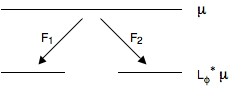
\includegraphics[width=2in]{IFSpush.jpg} 
   \caption{``IFS pushforward"}
   \label{figIFS}
\end{figure}

There are now two ways to push forward a measure $ \mu $ on $ X_1\cup\dots\cup X_N $:
\begin{enumerate}

\item \emph{Pushforward via the dynamics operator}: $ \mu \mapsto f_{\#}\mu $.  

This gives a measure supported on $ X $, or on $ E $ if $ \mu $ is supported on $ E $.

\item \emph{Pushforward via the IFS}: (see Figure \ref{figIFS})
\begin{equation} \label{pfif} 
\mu \mapsto   L_\phi^* \mu  :=  \sum_i F_{i\#} (\theta_i   \mu ) 
 = \sum_i\theta_i \circ   f \, F_{i\#}\mu
 = e^ \phi \sum_i   F_{i\#} \mu \text{ (from \eqref{pfifs})}.
\end{equation} 
The second equality follows from
\[
F_{i\#}(h\mu) = h \circ F_i^{-1}\, F_{i\#}\mu = h\circ f \, F_{i\#}\mu,
\]
using the fact  $ F_i:X\to X_i $ is one-one and onto.

\end{enumerate} 
The reason for the notation $ L_\phi^* $ is that this operator is the dual of a corresponding operator $ L_\phi  $ on continuous functions, see \eqref{adjo}.

\medskip \emph{Informal description}:  $ L^*_\phi \mu $ is obtained by taking all measures  $ F_{i\#} \mu $ obtained by pushing forward $ \mu $ with $ F_{i\#} $, and then weighting them by $ e^\phi  $ (i.e.\ by $ \theta_i\circ f $).

 The only difference with  pushing forward a mass distribution by a standard IFS  is that here the weights may vary over the space and the total mass is not necessarily conserved.

%%%%%%%%%%%%%%%%%%%%%%%
\subsection{The Adjoint Operators on Functions}
Note that 
\begin{equation} \label{}
\begin{aligned}
\int h \, df_{\#}\mu &= \int h\circ f  \, d\mu , \\
\int h \, d(L_\phi^*\mu) &= \sum_i \int h \, d(e^\phi F_{i\#}\mu)
   =   \sum_i \int e^{\phi\circ F_i}  \, h\circ F_i    \, d\mu ,
   \end{aligned} 
   \end{equation} 
by \eqref{pfif}.   See also Section~\ref{rto}.

\bigskip It follows that the two pushforward operators are the adjoints of the two operators $ \mathcal{C} (X) \to \mathcal{C} (X) $ given by
\begin{equation} \label{adjo}
\begin{aligned}
h &\mapsto h \circ f, \\
h & \mapsto L_\phi h  := \sum_i e^{\phi\circ F_i}  \, h\circ F_i  = \sum_i \theta_i\,  h\circ F_i .
 \end{aligned} 
\end{equation} 
The operator $ L_\phi$ is also called the \emph{(Ruelle) transfer operator}.

\bigskip The nicer of the  two operators is the second, essentially because the $ F_i $ are contractive, whereas $ f $ is expansive.

\bigskip \emph{Informal description} The graph of $ L_\phi h $ is obtained by taking the component of $ h $ over each $ X_i  $, rescaling back to the domain $ X $, weighting by $ \theta_i$, and adding the results.

\bigskip In the usual IFS case the \emph{probabilistic interpretation} is 
\[ L_\phi h (x) = \mathbb{E} ^x(X_1), \]
where $ (X_n)_{n\geq 1}  $ are iid random variables with 
\[  X_0 = x , \quad P(X_{n+1}= F_i y \mid  X_n = y) = \theta_i(y). \]
In the current situation we need to generalise this idea to a type of process with probabilities/intensities not necessarily summing to one. 


%%%%%%%%%%%%%%%%%%%%%%%%%
\subsection{Properties of the Transfer Operator}
It follows easily from the IFS interpretation, or see Section~\ref{rto}, that%
\footnote{For example in the case of $ L^{*2}_\phi$, using \eqref{pfif} twice,
\[
L^{*2}_\phi\mu  = e^\phi \sum_i F_{i\#}\left( e^\phi\sum_jF_{j\#} \mu \right)  
  = e^\phi e^{\phi\circ f} \sum_{i,j} F_{ij\#}\mu 
   = e^{S_2 \phi}  \sum_{i,j} F_{ij\#}\mu .
\]
Similarly for $ L^{*k}_\phi$.}
\footnote{In the case of  $L^2_\phi$, using  \eqref{adjo} twice,  
\[
L^2_\phi  h = L_\phi\left(\sum_ie^{\phi\circ F_i}h\circ F_i\right)
= \sum_i\sum_j e^{\phi\circ F_j}e^{\phi\circ F_i \circ F_j} h\circ F_i\circ F_j 
= \sum_{i,j} e^{S_2(\phi\circ F_{ij})}h\circ F_{ij}.
\]
Similarly for $ L^{k}_\phi$.   
Alternatively, by duality,
\[ 
\int L^k_\phi h \, d\mu = \int h \,  d\left( L^{*k}_\phi \mu\right) 
= \sum_{|w|=k} h  e^{S_k\phi}\, dF_{w\#}\mu 
= \sum_{|w|=k} h \circ F_w\, e^{S_k\phi\circ F_w}  d \mu .
\] 
}
\begin{equation} \label{itto}
\begin{aligned} 
L_\phi^{*k}  \mu &= e^{S_k\phi}\sum_{\{w:|w|=k\}}F_{w\#}\mu,\\
 L_\phi^{k}  h &= \sum_{\{w:|w|=k\}}e^{(S_k\phi)\circ F_w  }\, h\circ F_ w .
\end{aligned} 
\end{equation} 

Thus $ L^{*k}_\phi \mu $ is obtained by adding $ N^k $ disjoint contracted  copies    of $ \mu$ and reweighting by the function $ e^{S_k \phi } $.
The graph of $ L^k_\phi h $ is obtained by taking  $ N^k $ disjoint pieces of the graph of $ h $, expanding to the common domain $ X $, and reweighting each by $  e^{(S_k\phi)\circ F_w  } $.

\medskip
Fix $ w $ with $ |w|=k$. It follows from \eqref{itto} on replacing $ h $ by $ e^{-S_k\phi}h$, that
\begin{equation} \label{spsw}
\spt h \subset X_w \Longrightarrow h \circ F_w = L^k_\phi \left(e^{-S_k\phi}h \right),
\end{equation}
since only one term on the right side of the second equality in~\eqref{itto} is non zero.

\medskip
Finally,
\begin{equation} \label{}
\begin{aligned} 
\Big(L_\phi\big((h_1\circ f)\times h_2\big) \Big)(x) 
   &= \sum_i h_1(f\circ F_ix)\, h_2(F_i x)\, \theta_i(x) \\
   &= \sum_i h_1(x)\, h_2(F_ix)\, \theta_i(x) \\
    &= h_1(x)\times \big(L_\phi h_2\big)(x).
\end{aligned} 
 \end{equation} 

\begin{remark} ***Context later***
\begin{proposition} If $ \mu $ is IFS invariant with e-value $ \lambda $  then $ \lambda = P(\phi) $.
\end{proposition}

\begin{proof}
  Let $ h = \mathcal{X} _{E_w} $ where $ |w|=k $.  Then from~\eqref{spsw} since $ h \circ F_w = \mathcal{X}_E $,
\[
1 = \int h \circ F_w \, d\mu  = \int L^k_\phi \left( e^{-S_k\phi}h\right) d \mu \
= \int_{E_w} e^{-S_k\phi} d \left(L^{*k}_\phi \mu\right) = \lambda ^k \int_{E_w} e^{-S_k\phi} d\mu.
\]
 From Proposition \ref{prpbv} or  \eqref{PrBV}, if $ x_w \in E_w $, then 
 \begin{align*}  
e^{-M} e^{S_k\phi(x_w)} &\leq \lambda ^k \mu (E_w) \leq e^{M} e^{S_k\phi(x_w)},\\
\therefore\  
 e^{-M} \sum_{|w|=k} e^{S_k\phi(x_w)} &\leq \lambda ^k   \leq e^{M}  \sum_{|w|=k} e^{S_k\phi(x_w)},\\
\therefore\   -\frac{M}{k} +\frac{1}{k}\log  e^{-M} \sum_{|w|=k} e^{S_k\phi(x_w)} &\leq \lambda  \leq 
         \frac{M}{k} +  +\frac{1}{k} \log \sum_{|w|=k} e^{S_k\phi(x_w)}.\\
 \end{align*} 
Taking $ k \to \infty $ and using Definition~\ref{dfpg},  $ P(\phi) =  \lambda $.
 \end{proof} 
 
 Note that this shows directly that the limit in Definition~\ref{dfpg} exists, without the need for a subadditivity argument.
\end{remark} 


  
  

%%%%%%%%%%%%%%%%%%%%%%%%%%%%%%%%%%%%
\section{\textbf{Shannon Breiman McMillan Theorem}}  
A good reference for the following and consequences is \cite{Bil}*{Ch 5}.  See also \cite{Wal}*{thm 4.17, p95}.


\begin{theorem}
Suppose $ E_n(x) $ is the set in the partition $ \bigvee_{i=0}^{n-1} T^{-i}\alpha  $ containing $ x $.
Equivalently, $ E_n = A_{i_0}\cap\dots \cap A_{i_{n-1}} $ where $ A_{i_j} $ is the set in $ \alpha $ to which $ T^i x$ belongs.

Then
\[
-\frac{1}{n}\log \mu(E_n(x)) \to h(T,\alpha) 
\]
a.s.\ and in $ L^1 $.
\end{theorem}
 
See also \cite{Bil}*{Ch 5} for applications to dimensions.

*** More to come ***



%%%%%%%%%%%%%%%%%%%%%%%%%%%%%%%%%%%%
\section{\textbf{Variational Principle}}  

This connects the topological and measure theoretic entropies.  It parallels certain results on dimensions, see \cite{Bed}.

It extends to a  similar result for pressure.  For proofs at this stage see \cite{Wal}*{p189--191, 218--221} , following the method of \cite{Mis1}.

%%%%%%%%%%%%%%%%%%%%%%%%%%%%%%%%%%%%
%%%%%%%%%%%%%%%%%%%%%%%%%%%%%%%%%%%%
%%%%%%%%%%%%%%%%%%%%%%%%%%%%%%%%%%%%
\section{\textbf{Ruelle Perron Frobenius Theorem}}   \label{PFT}


\[  i \amalg j, \quad i \uplus j, \quad i \Cup j . \]




%%%%%%%%%%%%%%%%%%%%%%%%%%%%%%%%
%%%%%%%%%%%%%%%%%%%%%%%%%%%%%%%%
%%%%%%%%%%%%%%%%%%%%%%%%%%%%%%%%
%%%%%%%%%%%%%%%%%%%%%%%%%%%%%%%%


\begin{thebibliography}{9} 

\bib{Bed}{article}{
   author={Bedford, Tim},
   title={Applications of dynamical systems theory to fractals---a study of
   cookie-cutter Cantor sets},
   conference={
      title={Fractal geometry and analysis},
      address={Montreal, PQ},
      date={1989},
   },
   book={
      series={NATO Adv. Sci. Inst. Ser. C Math. Phys. Sci.},
      volume={346},
      publisher={Kluwer Acad. Publ.},
%      place={Dordrecht},
   },
   date={1991},
   pages={1--44},
%   review={\MR{1140719}},
}

\bib{Bil}{book}{
   author={Billingsley, Patrick},
   title={Ergodic theory and information},
   publisher={John Wiley \& Sons Inc.},
%   place={New York},
   date={1965},
   pages={xiii+195},
%   review={\MR{0192027 (33 \#254)}},
}

\bib{Boyd}{article}{
   author={Boyd, Stephen},
   title={Perron Frobenius Theory},
  note={Online Notes, Chapter 17 of course notes} 
     }


\bib{Boy}{article}{
   author={Boyle, Mike},
   title={Notes on the Perron-Frobenius Theory of Nonnegative matrices},
  note={Online Notes} 
     }


\bib{Bri}{book}{
   author={Brin, Michael},
   author={Stuck, Garrett},
   title={Introduction to dynamical systems},
   publisher={Cambridge University Press},
   place={Cambridge},
   date={2002},
   pages={xii+240},
%   isbn={0-521-80841-3},
%   review={\MR{1963683 (2003m:37001)}},
}
	
\bib{Edg}{book}{
   author={Edgar, Gerald A.},
   title={Measure, topology, and fractal geometry},
   series={Undergraduate Texts in Mathematics},
   publisher={Springer-Verlag},
   place={New York},
   date={1990},
   pages={xiv+230},
%   isbn={0-387-97272-2},
%   review={\MR{1065392 (92a:54001)}},
}

\bib{Fal}{book}{
   author={Falconer, Kenneth},
   title={Techniques in fractal geometry},
   publisher={John Wiley \& Sons Ltd.},
%   place={Chichester},
   date={1997},
   pages={xviii+256},
%   isbn={0-471-95724-0},
%   review={\MR{1449135 (99f:28013)}},
}

\bib{Kea}{article}{
   author={Keane, Michael S.},
   title={Ergodic theory and subshifts of finite type},
   conference={
      title={Ergodic theory, symbolic dynamics, and hyperbolic spaces
      (Trieste, 1989)},
   },
   book={
      series={Oxford Sci. Publ.},
      publisher={Oxford Univ. Press},
%      place={New York},
   },
   date={1991},
   pages={35--70},
%   review={\MR{1130172}},
}

\bib{Kea72}{article}{
   author={Keane, Michael},
   title={Strongly mixing $g$-measures},
   journal={Invent. Math.},
   volume={16},
   date={1972},
   pages={309--324},
%   issn={0020-9910},
%   review={\MR{0310193 (46 \#9295)}},
}

\bib{MW}{article}{
   author={Mauldin, R. Daniel},
   author={Williams, S. C.},
   title={Hausdorff dimension in graph directed constructions},
   journal={Trans. Amer. Math. Soc.},
   volume={309},
   date={1988},
%   number={2},
   pages={811--829},
%   issn={0002-9947},
%   review={\MR{961615 (89i:28003)}},
}


\bib{Mil}{article}{
   author={Milnor, John},
   title={Dynamics: Introductory Lectures},
  note={Preliminary Notes} 
     date={2001}
     }

%\bib{Mis1}{article}{
%   author={Misiurewicz, Micha{\l}},
%   title={A short proof of the variational principle for a ${\bf
%   Z}\sb{+}\sp{N}$ action on a compact space},
%   conference={
%      title={},
%      address={Rennes},
%      date={1975},
%   },
%   book={
%      publisher={Soc. Math. France},
% %     place={Paris},
%   },
%   date={1976},
%   pages={147--157. Ast\'erisque, No. 40},
%%   review={\MR{0444904 (56 \#3250)}},
%}
	

\bib{Mis1}{article}{
   author={Misiurewicz, M.},
   title={A short proof of the variational principle for a $Z\sp{n}\sb{+}$\
   action on a compact space},
 %  language={English, with Russian summary},
   journal={Bull. Acad. Polon. Sci. S\'er. Sci. Math. Astronom. Phys.},
   volume={24},
   date={1976},
%   number={12},
   pages={1069--1075},
%   issn={0001-4117},
 %  review={\MR{0430213 (55 \#3220)}},
}
		



\bib{PY}{book}{
   author={Pollicott, Mark},
   author={Yuri, Michiko},
   title={Dynamical systems and ergodic theory},
   series={London Mathematical Society Student Texts},
   volume={40},
   publisher={Cambridge University Press},
%   place={Cambridge},
   date={1998},
   pages={xiv+179},
%   isbn={0-521-57294-0},
%   isbn={0-521-57599-0},
%   review={\MR{1627681 (99f:58130)}},
}
	




\bib{Walop}{article}{
   author={Walters, Peter},
   title={Ruelle's operator theorem and $g$-measures},
   journal={Trans. Amer. Math. Soc.},
   volume={214},
   date={1975},
   pages={375--387},
%   issn={0002-9947},
%   review={\MR{0412389 (54 \#515)}},
}
		

\bib{Walvp}{article}{
   author={Walters, Peter},
   title={A variational principle for the pressure of continuous
   transformations},
   journal={Amer. J. Math.},
   volume={97},
   date={1975},
   number={4},
   pages={937--971},
%   issn={0002-9327},
%   review={\MR{0390180 (52 \#11006)}},
}
		

\bib{Wal}{book}{
   author={Walters, Peter},
   title={An introduction to ergodic theory},
   series={Graduate Texts in Mathematics},
   volume={79},
   publisher={Springer-Verlag},
%   place={New York},
   date={1982},
   pages={ix+250},
%   isbn={0-387-90599-5},
%   review={\MR{648108 (84e:28017)}},
}

\bib{Wil}{article}{
   author={Williams, Susan G.},
   title={Introduction to symbolic dynamics},
   conference={
      title={Symbolic dynamics and its applications},
   },
   book={
      series={Proc. Sympos. Appl. Math.},
      volume={60},
      publisher={Amer. Math. Soc.},
%      place={Providence, RI},
   },
   date={2004},
   pages={1--11},
%   review={\MR{2078843 (2005e:37024)}},
}
		
\bib{You}{article}{
   author={Young, Lai-Sang},
   title={Entropy in dynamical systems},
   conference={
      title={Entropy},
   },
   book={
      series={Princeton Ser. Appl. Math.},
      publisher={Princeton Univ. Press},
      place={Princeton, NJ},
   },
   date={2003},
   pages={313--327},
%   review={\MR{2035829 (2004k:37010)}},
}

	

\end{thebibliography}

\end{document} 

